\blankpage

\chapter{Projection onto the Laplacian space}

This chapter is devoted to the projection onto the space of Laplacian matrices, a problem that naturally arises in many graph learning algorithms as a key computational step. In several formulations, intermediate updates do not automatically satisfy the structural constraints of a valid Laplacian, making projection onto the Laplacian space necessary to enforce properties such as symmetry, zero row sums, and nonpositive off-diagonal entries. We argue that this projection step is sufficiently rich and nontrivial to warrant dedicated study, as its formulation, algorithmic realization, and numerical behavior significantly impact the overall performance of graph learning methods. Accordingly, this chapter presents and compares different algorithms for projecting onto the space of Laplacians, with particular attention to their computational complexity and convergence properties.

\section{Problem formulation}

The problem that we will be studying in this chapter is the quadratic projection onto the space of Laplacian matrices
\begin{equation}\label{eq:qlap_proj}
	\hat\L = \argmin_{\L\in\mathcal{L}} \Tr(\L\F) + \frac{\beta}{2}\norm{\L}_F^2
\end{equation}
where $\F\in\R^{D\times D}$ is a constant matrix, $\beta>0$ is a regularization parameter that controls the volume of the graph, and $\mathcal{L}\coloneqq\{\L:\ \L\succcurlyeq \mathbf{0}, [\L]_{ij}\leq 0\ \forall i\neq j, \L\mathbf{1}=\mathbf{0}\}$ denotes the set of $D\times D$ Laplacian matrices. Due to the symmetry of $\L$, the number of unknowns is $D_+\coloneqq D(D+1)/2$ corresponding to the entries on and below the diagonal. Therefore, we solve for the half-vectorization of $\L$ as suggested in~\cite{dong2016learning}, which is obtained by vectorizing its lower triangular part. The vectorization of $\L$ is denoted by $\l\coloneqq \text{vec}(\L)\in\R^{D^2}$, and the half-vectorization by $\lh\coloneqq \text{vech}(\L)\in\R^{D_+}$, which can be converted to $\l$ using the duplication matrix $\D\in\{0,1\}^{D^2\times D_+}$ as $\l = \D\lh$. Now, by using the fact that $\norm{\L}_F^2=\l^\top\l$ and $\Tr (\L\F)=\f^\top\l$, where $\f\coloneqq \text{vec}(\F)$, problem~\eqref{eq:qlap_proj} can be cast as a constrained quadratic program
\begin{equation}
	\label{eq:lap_est_qp} 
	\hat{\lh} = \argmin_{\lh\in\R^{D_+}} \frac{1}{2}\lh^\top\P\lh - \q^\top\lh\quad \text{s. t.}\ \A\lh = \b,\ \B\lh \leq \mathbf{0}
\end{equation}
where $\P\coloneqq \beta\D^\top\D$ and $\q\coloneqq \M^\top\f$. Matrix $\A\in\{0,1\}^{(D+1)\times D_+}$ handles the equality constraints $\L\mathbf{1}=\mathbf{0}$ and $\Tr(\L)=V$, and has the following structure
\setlength\delimitershortfall{-2pt}
\begin{equation}
	\A\coloneqq
	\left[
	\vcenter{\hbox{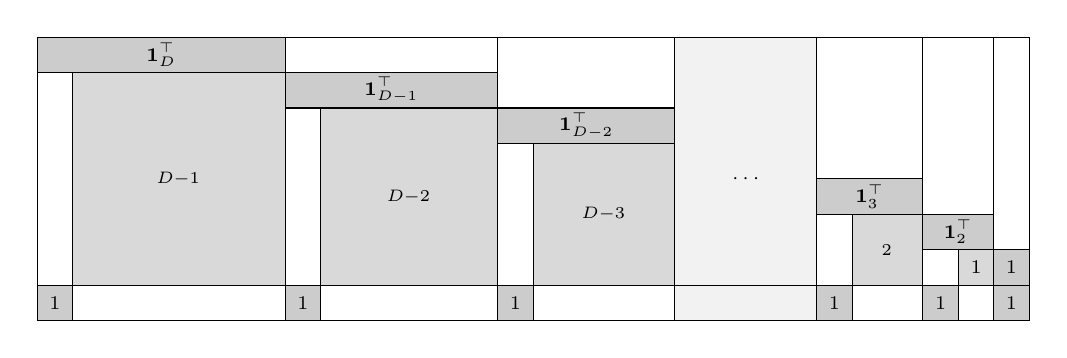
\begin{tikzpicture}[
		baseline=(current bounding box.center),
		scale=0.15,
		font=\scriptsize
	]
		\def\D{7}                 % change to any D >= 3
		\def\barH{3}              % bar height = stagger = zero-col width = trace-cell size
		% wj = (D-j)*barH  (zero-column is barH wide, trace cell is barH x barH)
		% cj = barH * j*(2D-j+1)/2
		% Dplus = barH * D*(D+1)/2
		\pgfmathtruncatemacro{\Dplus}{\barH * \D * (\D+1) / 2}
		\pgfmathtruncatemacro{\Dmax}{\D-1}
		\pgfmathtruncatemacro{\thresh}{\D-4}

		% Global vertical extents
		\pgfmathsetmacro{\gbot}{-(\D+1)*\barH}  % trace row bottom
		\pgfmathsetmacro{\ybot}{-\D*\barH}      % trace row top = sub-block bottom

		% Padding
		\path (-0.8,0.8) -- (\Dplus+0.8,\gbot-0.8);

		% -------------------------------------------------
		% Draw blocks
		% -------------------------------------------------
		\foreach \j in {0,...,\Dmax} {
			% cj = barH*j*(2D-j+1)/2 ;  wj = (D-j)*barH
			\pgfmathtruncatemacro{\cj}{\barH * \j * (2*\D - \j + 1) / 2}
			\pgfmathtruncatemacro{\wj}{(\D-\j)*\barH}
			\pgfmathsetmacro{\ybar}{-\j*\barH}         % bar top
			\pgfmathsetmacro{\ysub}{-(\j+1)*\barH}     % bar bottom = sub-block top
			\pgfmathsetmacro{\ymid}{(\ybar+\ysub)/2}   % bar label centre
			\pgfmathtruncatemacro{\hsub}{\D-\j-1}      % identity size (rows = cols)

			\pgfmathtruncatemacro{\isshown}{(\j<3) || (\j>\thresh) ? 1 : 0}

			\ifnum\isshown=1
				% --- 1^T bar ---
				\fill[black!20] (\cj,\ysub) rectangle (\cj+\wj,\ybar);
				\draw (\cj,\ysub) rectangle (\cj+\wj,\ybar);
				\ifnum\j=0
					\node at (\cj+\wj/2,\ymid) {$\mathbf{1}_{D}^\top$};
				\else
					\ifnum\j<3
						\node at (\cj+\wj/2,\ymid) {$\mathbf{1}_{D-\j}^\top$};
					\else
						\pgfmathtruncatemacro{\jtil}{\D-\j};
						\ifnum\jtil>1
							\node at (\cj+\wj/2,\ymid) {$\mathbf{1}_{\jtil}^\top$};
						\else
							\node at (\cj+\wj/2,\ymid) {$1$};
						\fi
					\fi
				\fi

				% --- Zero column (barH wide) + Identity square (bottom-pinned) ---
				\ifnum\hsub>0
					\fill[black!0]  (\cj,\ybot)        rectangle (\cj+\barH,\ysub);
					\draw           (\cj,\ybot)        rectangle (\cj+\barH,\ysub);
					\fill[black!15] (\cj+\barH,\ybot)  rectangle (\cj+\wj,\ysub);
					\draw           (\cj+\barH,\ybot)  rectangle (\cj+\wj,\ysub);
					\ifnum\hsub>0
						\pgfmathtruncatemacro{\jid}{\j+1}
						% identity side = hsub*barH; centre = (cj+barH+side/2, (ysub+ybot)/2)
						\pgfmathsetmacro{\icx}{\cj + \barH + \hsub*\barH/2}
						\pgfmathsetmacro{\icy}{(\ysub+\ybot)/2}
						\ifnum\j=4
							\node[font=\small] at (\icx,\icy) {$\I_2$};
						\else
							\ifnum\j=5
								\node at (\icx,\icy) {$1$};
							\else
								\node[font=\small] at (\icx,\icy) {$\I_{D-\jid}$};
							\fi
						\fi
					\fi
				\fi

				% --- Trace cell: barH x barH square, pinned to global bottom ---
				\fill[black!20] (\cj,\gbot) rectangle (\cj+\barH,\ybot);
				\draw           (\cj,\gbot) rectangle (\cj+\barH,\ybot);
				\pgfmathsetmacro{\tcy}{(\gbot+\ybot)/2}
				\node at (\cj+\barH/2,\tcy) {$1$};
			\else
				% --- Skipped block ---
				\fill[black!5]  (\cj,0) rectangle (\cj+\wj,\gbot);
				\draw[black!20] (\cj,0) rectangle (\cj+\wj,\gbot);
			\fi
		}

		% -------------------------------------------------
		% "..." in the gap (only when D > 6)
		% -------------------------------------------------
		\ifnum2<\thresh
			% xgapstart = cj for j=3 = barH*3*(2D-3+1)/2 = 3*barH*(D-1)
			\pgfmathtruncatemacro{\xgapstart}{3 * \barH * (\D-1)}
			% xgapend = cj for j=thresh+1 = barH*(thresh+1)*(2D-thresh)/2
			\pgfmathtruncatemacro{\xgapend}{(\thresh+1) * \barH * (2*\D - \thresh) / 2}
			\pgfmathtruncatemacro{\xgapmid}{(\xgapstart+\xgapend)/2}
			\pgfmathsetmacro{\ydots}{\gbot/2}
			\node at (\xgapmid, \ydots) {$\cdots$};
		\fi

		% -------------------------------------------------
		% Block boundaries and global horizontal lines
		% -------------------------------------------------
		\foreach \j in {0,...,\D} {
			\pgfmathtruncatemacro{\cj}{\barH * \j * (2*\D - \j + 1) / 2}
			\draw (\cj,0) -- (\cj,\gbot);
		}
		\draw (0,0)     -- (\Dplus,0);      % top
		\draw (0,\ybot) -- (\Dplus,\ybot);  % top of trace row
		\draw (0,\gbot) -- (\Dplus,\gbot);  % bottom
	\end{tikzpicture}}}
	\right]
\end{equation}

% \begin{equation}
% 	\A^\top\coloneqq
% 	\left[
% 	\vcenter{\hbox{\begin{tikzpicture}[
% 		baseline=(current bounding box.center),
% 		scale=0.15,
% 		font=\scriptsize
% 	]
% 		\def\D{7}
% 		\def\barH{3}
% 		\pgfmathtruncatemacro{\Dplus}{\barH * \D * (\D+1) / 2}
% 		\pgfmathtruncatemacro{\Wtot}{(\D+1) * \barH}
% 		\pgfmathtruncatemacro{\Wmain}{\D * \barH}
% 		\pgfmathtruncatemacro{\Dmax}{\D-1}
% 		\pgfmathtruncatemacro{\thresh}{\D-4}

% 		% Padding
% 		\path (-0.8,0.8) -- (\Wtot+0.8,-\Dplus-0.8);

% 		% -------------------------------------------------
% 		% Draw blocks
% 		% -------------------------------------------------
% 		\foreach \j in {0,...,\Dmax} {
% 			\pgfmathtruncatemacro{\rj}{\barH * \j * (2*\D - \j + 1) / 2}
% 			\pgfmathtruncatemacro{\hj}{(\D-\j)*\barH}
% 			\pgfmathtruncatemacro{\isshown}{(\j<3) || (\j>\thresh) ? 1 : 0}

% 			\ifnum\isshown=1
% 				% --- 1 bar (left) ---
% 				\fill[black!20] (\j*\barH,-\rj-\hj) rectangle (\j*\barH+\barH,-\rj);
% 				\draw (\j*\barH,-\rj-\hj) rectangle (\j*\barH+\barH,-\rj);
% 				\ifnum\j=0
% 					\node[rotate=90] at (\j*\barH+\barH/2,-\rj-\hj/2) {$\mathbf{1}_{D}$};
% 				\else
% 					\node[rotate=90] at (\j*\barH+\barH/2,-\rj-\hj/2) {$\mathbf{1}_{D-\j}$};
% 				\fi

% 				% --- Right part ---
% 				\ifnum\hj>\barH
% 					% Top row: zero strip
% 					\fill[black!0] (\j*\barH+\barH,-\rj-\barH) rectangle (\Wmain,-\rj);
% 					\draw (\j*\barH+\barH,-\rj-\barH) rectangle (\Wmain,-\rj);

% 					% Bottom: identity
% 					\fill[black!15] (\j*\barH+\barH,-\rj-\hj) rectangle (\Wmain,-\rj-\barH);
% 					\draw (\j*\barH+\barH,-\rj-\hj) rectangle (\Wmain,-\rj-\barH);

% 					% Identity label
% 					\pgfmathtruncatemacro{\hident}{\D-\j-1}
% 					\ifnum\hident>1
% 						\pgfmathtruncatemacro{\jid}{\j+1}
% 						\pgfmathsetmacro{\icx}{\j*\barH+\barH + \hident*\barH/2}
% 						\pgfmathsetmacro{\icy}{-\rj-\barH - \hident*\barH/2}
% 						\ifnum\j=4
% 							\node[font=\small] at (\icx,\icy) {$\I_2$};
% 						\else
% 							\node[font=\small] at (\icx,\icy) {$\I_{D-\jid}$};
% 						\fi
% 					\fi
% 				\else
% 					% No right part when hj == barH
% 				\fi
% 			\else
% 				% --- Skipped block ---
% 				\fill[black!5] (0,-\rj) rectangle (\Wmain,-\rj-\hj);
% 				\draw[black!20] (0,-\rj) rectangle (\Wmain,-\rj-\hj);
% 			\fi
% 		}

% 		% -------------------------------------------------
% 		\foreach \j in {0,...,\Dmax} {
% 			\pgfmathtruncatemacro{\isshown}{(\j<3) || (\j>\thresh) ? 1 : 0}
% 			\ifnum\isshown=1
% 				\pgfmathtruncatemacro{\rj}{\barH * \j * (2*\D - \j + 1) / 2}
% 				\fill[black!20] (\Wmain,-\rj-\barH) rectangle (\Wmain+\barH,-\rj);
% 				\draw (\Wmain,-\rj-\barH) rectangle (\Wmain+\barH,-\rj);
% 				\node at (\Wmain+\barH/2, -\rj-\barH/2) {$1$};
% 			\fi
% 		}


% % "..." in the gap
% 		% -------------------------------------------------
% 		\ifnum2<\thresh
% 			\pgfmathtruncatemacro{\ygapstart}{3 * \barH * (\D-1)}
% 			\pgfmathtruncatemacro{\ygapend}{(\thresh+1) * \barH * (2*\D - \thresh) / 2}
% 			\pgfmathtruncatemacro{\ygapmid}{(\ygapstart+\ygapend)/2}
% 			\pgfmathsetmacro{\xdots}{\Wtot/2}
% 			\node at (\xdots,-\ygapmid) {$\cdots$};
% 		\fi

% 		% -------------------------------------------------
% 		% Block boundaries and global edges
% 		% -------------------------------------------------
% 		\foreach \j in {0,...,\D} {
% 			\pgfmathtruncatemacro{\rj}{\barH * \j * (2*\D - \j + 1) / 2}
% 			\draw (0,-\rj) -- (\Wtot,-\rj);
% 		}
% 		\draw (0,0) -- (0,-\Dplus);
% 		\draw (\Wtot,0) -- (\Wtot,-\Dplus);
% 	\end{tikzpicture}}}
% 	\right]
% \end{equation}
Vector $\b\coloneqq[0,\ldots,0,V]^\top\in\R^{D+1}$, and matrix $\B\in\{0,1\}^{D_-\times D_+}$ handles the inequality constraints $[\L]_{ij}\leq0\ \forall i\neq j$ and has the following structure
% \begin{equation}
% 	\B\coloneqq \begin{tabular}{|c|c|c|c|c|c|c|c|c|c|c|}
% 		\hline
% 		$\mathbf{0}$ & $\I_{D-1}$ & \multicolumn{5}{c|}{$\mathbf{0}$}  & $\cdots$ & \multicolumn{3}{c|}{$\mathbf{0}$} \\ 
% 		\hline
% 		\multicolumn{2}{|c|}{$\mathbf{0}$} & $\mathbf{0}$ & \multicolumn{4}{c|}{$\I_{D-2}$}  & $\cdots$ & \multicolumn{3}{c|}{$\mathbf{0}$} \\ 
% 		\hline
% 		\multicolumn{3}{|c|}{$\mathbf{0}$} & $\mathbf{0}$ & \multicolumn{3}{c|}{$\I_{D-2}$}  & $\cdots$ & \multicolumn{3}{c|}{$\mathbf{0}$} \\ 
% 		\hline
% 		\multicolumn{4}{|c|}{$\mathbf{0}$} & $\mathbf{0}$ & $\cdots$ & \multicolumn{4}{c|}{$\mathbf{0}$} & \\ 
% 		\hline
% 	\end{tabular}
% \end{equation}
\begin{equation}
	\B\coloneqq
	\left[
	\vcenter{\hbox{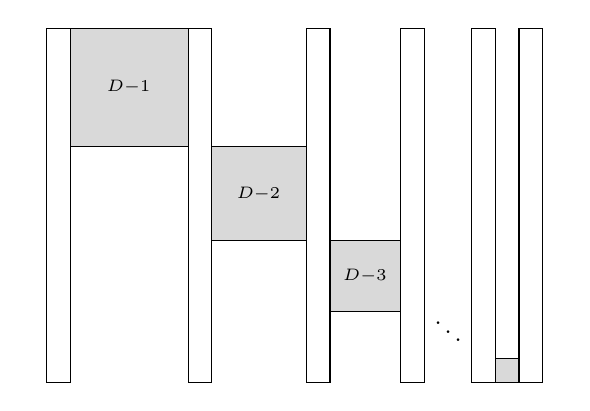
\begin{tikzpicture}[
		baseline=(current bounding box.center),
		scale=0.30,
		font=\small
	]
		\def\D{6}
		\pgfmathtruncatemacro{\Dminus}{\D*(\D-1)/2}
		\pgfmathtruncatemacro{\Dplus}{\D*(\D+1)/2}

		% -------------------------------------------------
		% Invisible padding: expand bounding box by 0.8 units
		% on each side so brackets don't touch the blocks.
		% Increase 0.8 for more margin, decrease for less.
		% -------------------------------------------------
		\path (-0.8,0) -- (\Dplus+0.8,-\Dminus);

		% Diagonal zero columns
		\foreach \k in {1,...,\D} {
			\pgfmathtruncatemacro{\c}{(\k-1)*(\D+1) - (\k-1)*\k/2}
			\fill[black!0] (\c,0) rectangle (\c+1,-\Dminus);
			\draw (\c,0) rectangle (\c+1,-\Dminus);
		}

		% First few identity blocks
		\def\numblocks{3}
		\foreach \k in {1,...,\numblocks} {
			\pgfmathtruncatemacro{\size}{\D-\k}
			\pgfmathtruncatemacro{\r}{(\k-1)*\D - (\k-1)*\k/2}
			\pgfmathtruncatemacro{\c}{\r+\k}

			\fill[black!15] (\c,-\r) rectangle (\c+\size,-\r-\size);
			\draw (\c,-\r) rectangle (\c+\size,-\r-\size);
			\node at (\c+\size/2,-\r-\size/2) {$\I_{D-\k}$};
		}

		% Dots
		\pgfmathtruncatemacro{\lastr}{(\numblocks)*\D - (\numblocks)*(\numblocks+1)/2}
		\pgfmathtruncatemacro{\lastc}{\lastr+\numblocks}
		\ifnum\lastr<\Dminus
			\node at ({(\lastc+\Dplus-1)/2-0.5},{(-\lastr-\Dminus)/2+1}) {$\ddots$};
		\fi

		% Last block
		\def\k{5}
		\pgfmathtruncatemacro{\size}{\D-\k}
		\pgfmathtruncatemacro{\r}{(\k-1)*\D - (\k-1)*\k/2}
		\pgfmathtruncatemacro{\c}{\r+\k}

		\fill[black!15] (\c,-\r) rectangle (\c+\size,-\r-\size);
		\draw (\c,-\r) rectangle (\c+\size,-\r-\size);
	\end{tikzpicture}}}
	\right]
\end{equation}
The projection onto the space of Laplacian matrices can be formulated as a quadratic program with linear constraints, making it a classical problem in the convex optimization literature. As such, it admits several well-established solution strategies, which we organize into two broad families. The \emph{second-order} family includes interior-point methods (IPM), which follow the central path of a barrier-augmented objective, and active-set methods, which exploit the sparsity of the optimal set of active inequality constraints. The \emph{first-order} family includes accelerated proximal gradient (APG) methods, which alternate gradient steps with projection onto the feasible set; the alternating direction method of multipliers (ADMM), which decouples the affine and conic constraints via variable splitting; and approaches based on the homogeneous self-dual embedding (HSDE), which additionally detects infeasibility within a parameter-free conic framework. Each of these techniques offers different trade-offs in terms of computational efficiency, scalability, and numerical robustness, and provides a principled framework for solving the projection problem to optimality.

\section{Interior-point method} 

The interior point method (IPM)~\cite{boyd2004convex} is a class of algorithms for solving convex optimization problems with inequality constraints by transforming the constrained problem into a sequence of unconstrained ones. This is achieved by incorporating the constraints into the objective through a barrier function, most commonly the logarithmic barrier, which penalizes proximity to the boundary of the feasible set and enforces strict feasibility of the iterates. Define the barrier function related to the inequality constraints $\B\lh\leq \mathbf{0}$
\begin{equation}
	\phi(\lh) = \sum_{i=1}^{D_-} -\log(-\b_i^\top\lh)
\end{equation}
where $\b_i\coloneqq[\B]_{i,:}$ denotes the $i^\text{th}$ row of $\B$. Define the extended objective function $g(\lh;t)\coloneqq tf(\lh) + \phi(\lh)$, where $t>0$ is a parameter that controls the weight of the original objective function $f(\lh)$. Starting with an initial guess $\lh_0\in\mathcal{H}$ (the strictly feasible interior of the feasible set) and a barrier parameter $t=t_0>0$, IPM solves the problem
\begin{equation}\label{eq:central_path}
	\lh_t = \argmin_{\lh\in\R^{D_+}} g(\lh;t)\quad \text{s. t.}\quad \A\lh = \b
\end{equation}
for a sequence of increasing value of $t\in\{t_1,t_2,\ldots,t_T\}$, typically obtained through the recursion $t_{k+1}=\mu t_k$, where $\mu>1$. By progressively increasing the barrier parameter, IPM generates a trajectory of solutions $p(t)\coloneqq g(\lh_t;t)$, known as the central path, that converges to the optimal solution of the original problem. A finite $t$ yields an $\mathcal{O}(m/t)$-accurate solution~\cite{ipm}. Therefore, increasing $t$ improves accuracy but increases computational cost. In fact, as $t\rightarrow\infty$, the solution of the barrier problem converges to the solution of the original problem. 

The resolution of the problem for a fixed $t_k$ is called the \emph{centering step}. In IPM, Newton's method is preferred over gradient descent for the centering step, due to the behavior of the barrier function, particularly near the boundary of the feasible region. As $\lh$ approaches the boundary of the feasible set for some $i\in\{1,\ldots,D_-\}$, $\b_i^\top\lh\longrightarrow0^-$. This causes the gradient $\nabla_{\lh} g(\lh;t)$ to grow arbitrarily large and point sharply away from the boundary, making gradient descent unstable and hard to tune near the feasible region's edges. Newton's method, in contrast, uses second-order information to adjust the step direction and step size. Near the boundary, the Hessian of the barrier function becomes large, and Newton's method naturally takes smaller, safer steps. Moreover, it follows the central path more faithfully than a steep gradient descent step would. The gradient of $g(\lh;t_k)$ is given by
\begin{equation*}
	\g_k(\lh)\coloneqq \nabla_{\lh} g(\lh;t_k) = t_k\P\lh - t_k\q + \sum_i\frac{\b_i}{-\b_i^\top\lh},
\end{equation*}
and the Hessian matrix by
\begin{equation*}
	\H_k(\lh)\coloneqq \Delta_{\lh} g(\lh;t_k) = t_k\P + \sum_i\frac{\b_i\b_i^\top}{(\b_i^\top\lh)^2}.
\end{equation*}
Using a warm start with $\lh_k^{(0)}=\lh_{k-1}$ from the previous centering step, the $l^\text{th}$ iteration of Newton's method for the $k^\text{th}$ centering step minimizes the second-order Taylor expansion around $\lh=\lh_k^{(l)}$
\begin{equation*}
	\tilde{\lh}_k^{(l)} = \argmin_{\lh\in\R^{D_+}} \frac{1}{2}\lh^\top \H_k^{(l)}\lh + (\g_k^{(l)} - \H_k^{(l)}\lh_k^{(l)})^\top\lh \quad \text{s.t.}\quad \A\lh = \b
\end{equation*}
where $\H_k^{(l)}\coloneqq \H_k(\lh_k^{(l)})$, and $\g_k^{(l)}\coloneqq \g_k(\lh_k^{(l)})$. Then, the full-step (candidate) Newton point $\tilde{\lh}_k^{(l)}$ and the associated dual variables $\tilde{\boldsymbol{\nu}}_k^{(l)}$ are given by the solution to the KKT system
\begin{equation*}
	\M_k^{(l)}\left [
	\begin{array}{c}
		\tilde{\lh}_k^{(l)} \\
		\tilde{\boldsymbol{\nu}}_k^{(l)} 
	\end{array}
	\right ] = 
	\left [
	\begin{array}{c}
		\H_k^{(l)}\lh_k^{(l)} - \g_k^{(l)} \\
		\b
	\end{array}
	\right ],\quad\text{where}\quad
	\M_k^{(l)}\coloneqq\left [
	\begin{array}{cc}
		\H_k^{(l)} & \A^\top \\
		\A & \mathbf{0}  
	\end{array}
	\right ],
\end{equation*}
and $\tilde{\boldsymbol{\nu}}_k^{(l)}\in\R^{D}$ are the dual variables of Lagrange multipliers. This solution ensures that the equality constraints are satisfied in each Newton iteration of the centering step, while the presence of the barrier function ensures that we stay inside the feasible region. A brute force approach to solve this system would be to invert $\M_k^{(l)}$. However, here we leverage the structure of this matrix using the Schur complement recursively to perform a more efficient computation of the solution. The Schur complement of $\M_k^{(l)}$ w.r.t. $\H_k^{(l)}$ is given by
\begin{equation}
	\M_k^{(l)}|\H_k^{(l)} = -\A(\H_k^{(l)})^{-1}\A^\top
\end{equation}
and the inverse of $\M_k^{(l)}$ can be expressed in terms of $\M_k^{(l)}|\H_k^{(l)}$ as
\begin{small}
	\begin{equation}\label{eq:Minv}
		(\M_k^{(l)})^{-1} = \left[
		\begin{array}{cc}
			(\H_k^{(l)})^{-1} - (\H_k^{(l)})^{-1}\A^\top\Rm_k^{(l)}  & \Rm_k^{(l)\top} \\
			\Rm_k^{(l)} & {(\M_k^{(l)}|\H_k^{(l)})}^{-1}
		\end{array}
		\right]
	\end{equation}
\end{small}%
where $\Rm_k^{(l)}\coloneqq -{(\M_k^{(l)}|\H_k^{(l)})}^{-1}\A(\H_k^{(l)})^{-1}$. Since $\lh^\top \P \lh= \beta \l^\top \l = \beta \norm{\L}_F^2$ and $\sum_i\frac{1}{(\b_i^\top\lh)^2}\b_i\b_i^\top$ is diagonal, it is not difficult to check that matrix $\H_k^{(l)}$ is diagonal and its elements have the following structure
\begin{align}
	&\H_k^{(l)}=\text{diag}(t_k\beta, \underbrace{2t_k\beta+\frac{1}{[\lh_k^{(l)}]_1^2},\ldots,2t_k\beta+\frac{1}{[\lh_k^{(l)}]_{D-1}^2}}_{D-1},t_k\beta,\ldots, \label{eq:ipm_delta} \\
	&\hspace{1.8cm}\underbrace{2t_k\beta+\frac{1}{[\lh_k^{(l)}]_{D+1}^2},\ldots,2t_k\beta+\frac{1}{[\lh_k^{(l)}]_{2D-1}^2}}_{D-2},t_k\beta,\ldots, t_k\beta,2t_k\beta+\frac{1}{[\lh_k^{(l)}]_{D_+-2}^2},t_k\beta) \nonumber
\end{align}
Therefore, inverting $\H_k^{(l)}$ only costs $\mathcal{O}(D_+)$. However, the Schur complement $\M_k^{(l)}|\H_k^{(l)}$ has no analytic expression because the diagonal elements of $\H_k^{(l)}$ are different in general. Therefore, since $\M_k^{(l)}|\H_k^{(l)}$ is a $D\times D$ matrix, its inversion costs $\mathcal{O}(D^3)$ in general. Still, this is far cheaper than the naive approach of inverting the full $(D_+ + D + 1)\times(D_+ + D + 1)$ matrix $\M_k^{(l)}$ to solve the KKT system, which would cost $\mathcal{O}\big((D_+ + D + 1)^3\big)$. 

The inner loop is terminated once the $l$-th Newton iterate is sufficiently close to the minimizer of the $k$-th barrier subproblem~\eqref{eq:central_path}. Because each Newton step solves the KKT system exactly, the equality constraint $\A\tilde{\lh}_k^{(l)}=\b$ holds by construction. The KKT solution defines the full-step Newton direction
\begin{equation}\label{eq:newton_direction}
	\Delta\lh_k^{(l)} \coloneqq \tilde{\lh}_k^{(l)} - \lh_k^{(l)}.
\end{equation}
Because both $\tilde{\lh}_k^{(l)}$ and $\lh_k^{(l)}$ satisfy the equality constraint, $\A\Delta\lh_k^{(l)}=\mathbf{0}$; therefore any update of the form
\begin{equation}\label{eq:damped_update}
	\lh_k^{(l+1)} = \lh_k^{(l)} + s_k^{(l)}\Delta\lh_k^{(l)},\qquad s_k^{(l)}\in(0,1],
\end{equation}
remains feasible for the equality constraints. The quality of the centering step is monitored through the Newton decrement
\begin{equation}\label{eq:newton_decrement}
	\omega(\lh_k^{(l)})^2 \coloneqq (\Delta\lh_k^{(l)})^{\top} \H_k^{(l)} \Delta\lh_k^{(l)} = -(\Delta\lh_k^{(l)})^{\top} \g_k^{(l)},
\end{equation}
and the inner loop stops as soon as $\omega(\lh_k^{(l)})\le\varepsilon_{\text{in}}$, where $\varepsilon_{\text{in}}$ is a small positive tolerance. Inside the quadratic convergence region the full step $s_k^{(l)}=1$ is taken. Otherwise the step size is reduced by backtracking line search until strict feasibility and sufficient decrease are attained:
\begin{subequations}\label{eq:backtracking_conditions}
\begin{align}
	\B\big(\lh_k^{(l)}+s\Delta\lh_k^{(l)}\big) &< \mathbf{0}, \label{eq:backtracking_feas}\\
	g\big(\lh_k^{(l)}+s\Delta\lh_k^{(l)};t_k\big) &\le g\big(\lh_k^{(l)};t_k\big) - \alpha s\,\omega(\lh_k^{(l)})^2, \label{eq:backtracking_armijo}
\end{align}
\end{subequations}
with $\alpha\in(0,1/2)$. Starting from $s=1$ and multiplying by $\beta_\text{ls}\in(0,1)$ until both conditions hold yields a step that monotonically decreases the barrier objective. The right-hand side of~\eqref{eq:backtracking_armijo} is exactly the first-order decrease predicted by the quadratic model, as encoded in the second equality of~\eqref{eq:newton_decrement}. Consequently, when $\omega(\lh_k^{(l)})\le\eta$ for the constant $\eta$ of Theorem~\ref{thm:newton_conv}, the backtracking procedure accepts $s=1$ and the damped update reduces to the standard full Newton step.

\begin{algorithm}[t]
	\caption{Laplacian projection via IPM}
	\label{alg:backtrack}
	\begin{algorithmic}[1]
		\renewcommand{\algorithmicrequire}{\textbf{Input:}}
		\renewcommand{\algorithmicensure}{\textbf{Output:}}
		\Require Strictly feasible initial value $\lh_0\in\mathcal{H}$; regularization parameter $\beta>0$; constant diagonal matrix $\P\in\R^{D\times D}$; constant vector $\q\in\R^{D_+}$; constraint matrices $\A$ and $\B$; initial barrier parameter $t_0>0$; multiplier constant $\mu>1$; outer loop tolerance $\varepsilon_\text{out}>0$; inner loop tolerance $\varepsilon_\text{in}>0$; inner loop maximum number of iterations $I_\text{in}$; backtracking parameters $\alpha\in(0,1/2)$ and $\beta_\text{ls}\in(0,1)$.
		\Ensure Solution $\lh$.
		\State $t\gets t_0$, $\lh\gets \lh_0$
		\While{$\frac{D_-}{t}>\varepsilon_\text{out}$}
		\Comment{Outer loop: central path}
		\State $\omega\gets \varepsilon_\text{in}+1$, $l\gets 1$
		\While{$\omega>\varepsilon_\text{in}$\textbf{ and }$l<I_\text{in}$}
		\Comment{Inner loop: centering step}
		\State $\g \gets t\P\lh - t\q + \sum_i\frac{\b_i}{-\b_i^\top\lh}$
		\State $\H\gets t\P + \sum_i\frac{\b_i\b_i^\top}{(\b_i^\top\lh)^2}$
		\State $\H^{-1}\gets (\H)^{-1}$
		\State $\M|\H\gets -\A\H^{-1}\A^\top$
		\State $\Rm\gets -(\M|\H)^{-1}\A\H^{-1}$
		\State $\M^{-1} \gets \left[
		\begin{array}{cc}
			\H^{-1} - \H^{-1}\A^\top\Rm  & \Rm^\top \\
			\Rm & (\M|\H)^{-1}
		\end{array}
		\right]$
		\State $[\lh^+, \boldsymbol{\nu}]^\top \gets \M^{-1}[\H\lh-\g,\b]^\top$
		\State $\Delta\lh \gets \lh^+ - \lh$
		\State $\omega\gets\sqrt{(\Delta\lh)^\top\H\Delta\lh}$
		\State $s\gets 1$
		\While{$\max_i \b_i^\top(\lh+s\Delta\lh)\ge 0$ \textbf{or} $g(\lh+s\Delta\lh;t)>g(\lh;t)-\alpha s\omega^2$}
		\Comment{Backtracking line search}
		\State $s\gets \beta_\text{ls} s$
		\EndWhile
		\State $\lh\gets \lh+s\Delta\lh$
		\State $l\gets l+1$
		\EndWhile
		\State $t\gets \mu t$
		\EndWhile
		\Return $\lh$
	\end{algorithmic} 
\end{algorithm}

\subsection{Convergence analysis}
\label{sec:ipm_conv_analysis}

The convergence behavior of Algorithm~\ref{alg:backtrack} can be characterized in two stages: the outer iterations along the central path, and the inner Newton iterations within each centering step. We follow the analysis framework of~\cite{ipm,nesterov1994interior}, particularized here to the QP in~\eqref{eq:lap_est_qp}. The analysis relies on the following assumptions.

\begin{assumption}\label{ass:ipm_strict_feas}
	The QP in~\eqref{eq:lap_est_qp} is strictly feasible, i.e., the open set $\mathcal{H}\coloneqq\{\lh\in\R^{D_+}: \A\lh=\b,\ \B\lh<\mathbf{0}\}$ is non-empty.
\end{assumption}
\begin{assumption}\label{ass:ipm_full_rank}
	The equality-constraint matrix $\A$ has full row rank.
\end{assumption}
\begin{assumption}\label{ass:ipm_pd}
	The Hessian of the objective $\P$ is positive definite, $\P\succ\mathbf{0}$, and the optimal value $p^\ast\coloneqq f(\hat{\lh})$ of~\eqref{eq:lap_est_qp} is finite and attained.
\end{assumption}
\noindent Assumption~\ref{ass:ipm_strict_feas} (Slater's condition) ensures that the barrier $\phi$ has a non-empty open domain on the equality-constrained set, so the central path is well-defined for every $t>0$. The Laplacian $\L$ of any connected graph with edge weights in $(0,V/D_-)$ has strictly negative off-diagonal entries, $\Tr(\L)=V$, and $\L\mathbf{1}=\mathbf{0}$, hence its half-vectorization belongs to $\mathcal{H}$ and Assumption~\ref{ass:ipm_strict_feas} holds. Assumption~\ref{ass:ipm_full_rank} is satisfied by construction of $\A$, as discussed in Section~\ref{sec:conv_analysis}. Finally, $\P=\beta\D^\top\D$ with $\beta>0$ and $\D$ has full column rank, so $\P\succ\mathbf{0}$ and Assumption~\ref{ass:ipm_pd} holds; existence of $\hat{\lh}$ follows from continuity of $f$ and compactness of the sublevel sets of $f$ on the closed feasible set, guaranteed by $\P\succ\mathbf{0}$.

\paragraph{Outer-loop convergence.} The fundamental property of the central path is that the distance to the optimal value $p^\ast$ decays with $1/t$.

\begin{lemma}[$\text{Duality gap~\cite[\S11.2]{ipm}}$]\label{lemma:duality_gap}
	Under Assumptions~\ref{ass:ipm_strict_feas}--\ref{ass:ipm_pd}, the central-path point $\lh_t$ defined by~\eqref{eq:central_path} satisfies
	\begin{equation}\label{eq:duality_gap}
		0\leq f(\lh_t) - p^\ast \leq \frac{D_-}{t}.
	\end{equation}
\end{lemma}
Lemma~\ref{lemma:duality_gap} justifies the outer-loop stopping criterion $D_-/t\leq \varepsilon_\text{out}$ used in Algorithm~\ref{alg:backtrack}: any iterate satisfying it is $\varepsilon_\text{out}$-suboptimal in objective value. Because $t$ grows geometrically, the number of outer iterations to reach a target accuracy is logarithmic.

\begin{theorem}[$\text{Outer-loop iteration count~\cite[\S11.3]{ipm}}$]\label{thm:outer_convergence}
	Let $\varepsilon_\text{out}>0$, $t_0>0$, and $\mu>1$. Under Assumptions~\ref{ass:ipm_strict_feas}--\ref{ass:ipm_pd}, Algorithm~\ref{alg:backtrack} produces an $\varepsilon_\text{out}$-suboptimal feasible iterate after at most
	\begin{equation}\label{eq:outer_iters}
		K_\text{out} = \left\lceil \frac{\log\!\left(D_-/(t_0\varepsilon_\text{out})\right)}{\log\mu}\right\rceil
	\end{equation}
	outer iterations.
\end{theorem}

\paragraph{Inner-loop convergence.} The Newton inner-loop convergence proof of IPM is built on the self-concordance theory of Nesterov and Nemirovskii~\cite{nesterov1994interior}. Since self-concordance involves higher-order derivatives evaluated along a direction, we first recall the notion of a directional derivative. 
\begin{definition}[Directional derivative]\label{def:dir_deriv}
For a function $\psi: \R^D\to\R$ and a point $\lh\in\R^D$ in its domain, the directional derivative of $\psi$ at $\lh$ along a vector $\v$ is defined as
\begin{equation}
D_{\v}\psi(\lh)\coloneqq \lim_{t\to0} \frac{\psi(\lh+t\v)-\psi(\lh)}{t} = \nabla\psi(\lh)^\top\v = \sum_i \frac{\partial\psi(\lh)}{\partial \lambda_i}v_i.
\end{equation}
\end{definition}
The second and third order directional derivatives are obtained by successive application of the directional derivative operator
\begin{align}
D_{\v}^2 \psi(\lh) &\coloneqq D_{\v}[D_{\v}\psi(\lh)]
= \lim_{t\to0} \frac{D_{\v}\psi(\lh+t\v)-D_{\v}\psi(\lh)}{t}
= \v^\top\Delta\psi(\lh)\v=\sum_{i,j}\frac{\partial^2\psi(\lh)}{\partial \lambda_i\,\partial \lambda_j}\,v_i v_j, \\
D_{\v}^3 \psi(\lh) &\coloneqq D_{\v}[D_{\v}[D_{\v}\psi(\lh)]]
= \lim_{t\to0} \frac{D_{\v}^2\psi(\lh+t\v)-D_{\v}^2\psi(\lh)}{t}
= \sum_{i,j,k}\frac{\partial^3\psi(\lh)}{\partial \lambda_i\,\partial \lambda_j\,\partial \lambda_k}\,v_i v_j v_k.
\end{align}
where $\Delta\psi(\lh)\in\R^{D\times D}$ is the Hessian of $\psi$ at $\lh$. In general, the $k^\text{th}$-order directional derivative is obtained by multiplying each $k^\text{th}$-order partial derivative by the corresponding product of components of the direction vector and summing over all index combinations
\begin{equation}
	D_{\v}^k \psi(\lh) \coloneqq \sum_{i_1,\ldots,i_k=1}\frac{\partial^k\psi(\lh)}{\partial \lambda_{i_1}\cdots \partial \lambda_{i_k}}\,v_{i_1}\cdots v_{i_k}.
\end{equation}
\begin{definition}[Self-concordance of the barrier]
	A convex function $\psi:\mathcal{H}\rightarrow\R$, three times continuously differentiable, is \emph{self-concordant} if for all $\lh\in\mathcal{H}$ and all $\v\in\R^{D_+}$
\begin{equation}\label{eq:self_concord}
	|D_{\v}^3 \psi(\lh)|\leq 2\left(D_{\v}^2\psi(\lh)\right)^{3/2}.
\end{equation}
\end{definition}

\begin{lemma}\label{lemma:self_concord}
	The logarithmic barrier $\phi(\lh) = -\sum_{i=1}^{D_-}\log(-\b_i^\top\lh)$ is self-concordant on $\mathcal{H}$, and $g(\lh;t)\coloneqq tf(\lh)+\phi(\lh)$ is self-concordant on $\mathcal{H}$ for every $t>0$.
\end{lemma}
\begin{proof}
	The univariate function $u\mapsto -\log(u)$ on $u>0$ is self-concordant~\cite[Example 1]{nesterov1994interior}, and self-concordance is preserved under composition with affine maps and under summation on a common domain~\cite[Proposition 2.1.1]{nesterov1994interior}. Hence each term $-\log(-\b_i^\top\lh)$ is self-concordant on $\{\lh:\b_i^\top\lh<0\}$, and $\phi$ is self-concordant on the intersection $\mathcal{H}$. Since $tf(\lh)$ is a convex quadratic function, its third derivative vanishes identically, so the inequality~\eqref{eq:self_concord} for $\phi$ implies the same inequality for $g(\cdot;t)=tf(\cdot)+\phi(\cdot)$.
\end{proof}
Each centering step minimizes the self-concordant function $g(\cdot;t_k)$ over the affine set $\{\lh:\A\lh=\b\}$ via Newton's method, starting from the warm start $\lh_k^{(0)} = \lh_{k-1}$. The Newton decrement~\eqref{eq:newton_decrement} serves both as a measure of proximity to the centering optimum and as the standard inner-loop stopping criterion. Self-concordance yields the following two-phase characterization of Newton's method.

\begin{theorem}[Two-phase convergence of Newton's method for a self-concordant function {\cite[\S9.6.3--9.6.4]{ipm}}]\label{thm:newton_conv}
	There exist universal constants $0<\eta\leq 1/4$ and $c>0$ such that the following hold for the centering step applied to $g(\cdot;t_k)$ over the affine set $\{\lh:\A\lh=\b\}$.
	\begin{enumerate}[label=(\roman*)]
		\item \emph{Damped phase.}\label{it:damped_phase} If $\lh\in\mathcal{H}$ satisfies $\A\lh=\b$ and $\omega(\lh)\ge\eta$, then the damped Newton step
		\begin{equation}\label{eq:damped_newton_step}
			\lh^+ = \lh + \frac{1}{1+\omega(\lh)}\Delta\lh
		\end{equation}
		satisfies
		\begin{equation}\label{eq:damped_decrease}
			g(\lh^+;t_k) \le g(\lh;t_k) - \omega(\lh) + \log(1+\omega(\lh))
			\le g(\lh;t_k) - \eta + \log(1+\eta).
		\end{equation}
		\item \emph{Quadratic phase.}\label{it:quadratic_phase} If the centering step is initialized at any $\lh_k^{(0)}\in\mathcal{H}$ with $\A\lh_k^{(0)}=\b$ and $\omega(\lh_k^{(0)})\le\eta$, full Newton steps satisfy
		\begin{equation*}
			\omega(\lh_k^{(l+1)})\leq 2\,\omega(\lh_k^{(l)})^2,\qquad l=0,1,\dots
		\end{equation*}
		Consequently, the centering step terminates with $\omega(\lh_k^{(l)})\leq\varepsilon_\text{in}$ in at most
		\begin{equation}\label{eq:newton_iters}
			N_k \leq \log_2\log_2\frac{1}{\varepsilon_\text{in}} + c
		\end{equation}
		Newton iterations.
	\end{enumerate}
\end{theorem}
\begin{proof}
	For part~\ref{it:damped_phase}, because $g(\cdot;t_k)$ is self-concordant on $\mathcal{H}$ and $\Delta\lh$ lies in the nullspace of $\A$, the standard one-dimensional self-concordance bound applies along the feasible segment $\{\lh+s\Delta\lh:s\in[0,1]\}$. Taking $s=1/(1+\omega(\lh))$ gives the first inequality in~\eqref{eq:damped_decrease}; the second inequality follows because $\omega\mapsto \omega-\log(1+\omega)$ is increasing for $\omega>0$ and $\omega(\lh)\ge\eta$. For part~\ref{it:quadratic_phase}, the result follows from Lemma~\ref{lemma:self_concord} together with the standard local analysis of full-step Newton's method for self-concordant functions; see~\cite[\S9.6.4]{ipm}. The equality-constrained step in Algorithm~\ref{alg:backtrack} is the direct analogue restricted to the affine subspace $\{\lh:\A\lh=\b\}$.
\end{proof}

\noindent The damped phase guarantees a constant decrease of the barrier objective whenever the iterate lies outside the quadratic region. Since the objective is bounded below by the centering optimum $g(\lh_{t_k};t_k)$, the iterates enter $\mathcal{Q}_\eta$ after finitely many damped steps. Under the warm start, Lemma~\ref{lemma:warm_start} bounds the initial gap, so the number of damped steps per centering step is uniformly bounded by a constant depending only on $\mu$ and $\eta$.

\noindent The bound in~\eqref{eq:newton_iters} reflects the extremely fast quadratic phase. The \emph{quadratic convergence region} of the centering step is the set of strictly feasible points whose Newton decrement is below the constant $\eta$ of Theorem~\ref{thm:newton_conv},
\begin{equation}\label{eq:quad_region}
	\mathcal{Q}_\eta \coloneqq \{\lh\in\mathcal{H}:\A\lh=\b,\ \omega(\lh)\le\eta\}.
\end{equation}
Inside $\mathcal{Q}_\eta$, full Newton steps are guaranteed to decrease the Newton decrement quadratically, so the backtracking line search accepts $s=1$. Damped Newton steps are the standard tool when the initial point lies outside $\mathcal{Q}_\eta$; Algorithm~\ref{alg:backtrack} includes such a safeguard. Under the warm start $\lh_k^{(0)}=\lh_{k-1}$ the iterates typically lie inside the quadratic region, so full steps are accepted. If, on some iteration, the warm start were to give $\omega(\lh_k^{(0)})>\eta$ (and in particular if $\omega(\lh_k^{(0)})^2>1/2$), the quadratic bound would no longer apply and full steps would not be guaranteed to reduce the Newton decrement; the backtracking line search would then dampen the steps until the decrement drops below $\eta$.

The constant $\eta$ is a theoretical quantity furnished by the self-concordance analysis (one may take $\eta\le 1/4$), and it is \emph{not} required explicitly by Algorithm~\ref{alg:backtrack}. Operationally, the algorithm only monitors the computable Newton decrement $\omega(\lh_k^{(l)})$. A full step is attempted first; if the backtracking conditions~\eqref{eq:backtracking_conditions} accept $s=1$, the step is taken and the observed quadratic reduction of the decrement confirms that the iterate is in (or has entered) $\mathcal{Q}_\eta$. If $s=1$ is rejected, the line search produces a damped step that still decreases the barrier objective, thereby driving the iterates into $\mathcal{Q}_\eta$.

\begin{lemma}[Warm-start gap]\label{lemma:warm_start}
	Under Assumptions~\ref{ass:ipm_strict_feas}--\ref{ass:ipm_pd}, with the warm start $\lh_k^{(0)} = \lh_{k-1}=\lh_{t_{k-1}}$, the gap $g(\lh_k^{(0)};t_k) - g(\lh_{t_k};t_k)$ is bounded above by a constant $C(\mu)$ that depends on $\mu$ and $D_-$ but not on $k$.
\end{lemma}
\begin{proof}
	Since $g(\lh;t_k) = t_k f(\lh) + \phi(\lh)$ and $t_k=\mu t_{k-1}$, write
	\begin{equation*}
		g(\lh;t_k) = \mu g(\lh;t_{k-1}) + (1-\mu)\phi(\lh).
	\end{equation*}
	A direct computation using the duality bound of Lemma~\ref{lemma:duality_gap} and the optimality of $\lh_{t_{k-1}}$ for $g(\cdot;t_{k-1})$ on the affine set yields
	\begin{equation*}
		g(\lh_{t_{k-1}};t_k)-g(\lh_{t_k};t_k) \leq D_-(\mu - 1 - \log\mu),
	\end{equation*}
	independently of $k$; see~\cite[\S11.5.5]{ipm} for the algebraic details. Setting $C(\mu)\coloneqq D_-(\mu-1-\log\mu)$ proves the lemma.
\end{proof}

\paragraph{Overall iteration complexity.} Combining Lemma~\ref{lemma:warm_start} with Theorem~\ref{thm:newton_conv} bounds the inner-loop work uniformly in $k$, and Theorem~\ref{thm:outer_convergence} bounds the outer loop. The product yields the total complexity.

\begin{theorem}[Total iteration complexity]\label{thm:total_complexity}
	Under Assumptions~\ref{ass:ipm_strict_feas}--\ref{ass:ipm_pd}, Algorithm~\ref{alg:backtrack} produces an $\varepsilon_\text{out}$-suboptimal feasible solution in at most
	\begin{equation}\label{eq:total_iters}
		\left\lceil\frac{\log\!\left(D_-/(t_0\varepsilon_\text{out})\right)}{\log\mu}\right\rceil
		\left(\log_2\log_2\frac{1}{\varepsilon_\text{in}} + c(\mu)\right)
	\end{equation}
	total Newton iterations, where $c(\mu)>0$ is a constant depending on $\mu$ (and on $D_-$) but not on $k$.
\end{theorem}
\begin{proof}
	By Theorem~\ref{thm:outer_convergence} the outer loop performs at most $K_\text{out}$ iterations. For every outer iteration $k\geq 1$, Lemma~\ref{lemma:warm_start} bounds the warm-start gap by $C(\mu)=D_-(\mu-1-\log\mu)$. For a self-concordant function, a bounded initial gap implies a bounded initial Newton decrement, so after at most a constant number of (possibly damped) Newton steps the iterates enter the quadratic convergence region of Theorem~\ref{thm:newton_conv}. Hence the number of Newton iterations of the $k$-th centering step is uniformly bounded by $N_k\leq \log_2\log_2(1/\varepsilon_\text{in}) + c(\mu)$. Summing over $k=1,\ldots,K_\text{out}$ gives~\eqref{eq:total_iters}.
\end{proof}

Per Newton iteration, the dominant cost is the inversion of the Schur complement $\M_k^{(l)}|\H_k^{(l)}\in\R^{D\times D}$, which is $\mathcal{O}(D^3)$, while the diagonal Hessian $\H_k^{(l)}$ in~\eqref{eq:ipm_delta} is inverted in $\mathcal{O}(D_+)=\mathcal{O}(D^2)$. Combining with Theorem~\ref{thm:total_complexity}, the overall arithmetic cost of Algorithm~\ref{alg:backtrack} is
\begin{equation}\label{eq:ipm_total_cost}
	\mathcal{O}\!\left(\log\!\left(D_-/(t_0\varepsilon_\text{out})\right)\cdot D^3\right),
\end{equation}
where the dependence on $\mu$, $\gamma$, $c$, and $\varepsilon_\text{in}$ has been absorbed into the constant.

\paragraph{Choice of the multiplier $\mu$.} Theorem~\ref{thm:total_complexity} reveals the standard IPM trade-off: $K_\text{out}$ in~\eqref{eq:outer_iters} is decreasing in $\mu$, while the per-step warm-start gap $D_-(\mu-1-\log\mu)$ in Lemma~\ref{lemma:warm_start} is increasing in $\mu$. The product is relatively insensitive to $\mu$ over a wide range; in practice, $\mu\in[10,100]$ provides a robust trade-off~\cite[\S11.3.1]{ipm}.

\section{Active-set method}
\label{sec:active_set_method}

Active-set methods are a classical alternative to IPM for QPs with linear inequality constraints~\cite{nocedal2006numerical,goldfarb1983numerically}. They exploit the fact that the optimal solution lies on a face of the feasible polyhedron determined by the subset of inequality constraints that are active at the optimum. The method maintains a working estimate $\mathcal{W}\subseteq\{1,\ldots,D_-\}$ of this active set and updates it iteratively, adding or dropping a single constraint per iteration, until the KKT conditions are satisfied.

For the Laplacian projection problem~\eqref{eq:lap_est_qp}, the active inequalities at the solution $\hat{\lh}$ correspond to the off-diagonal entries that are zero, i.e., to the missing edges of the recovered graph. Since real-world graphs are typically sparse, $|\mathcal{W}_\ast|$ is large at the optimum, and the algorithm rapidly identifies the support of the graph; the remaining iterations refine the values of the non-zero edge weights. We adopt the dual active-set algorithm of Goldfarb and Idnani~\cite{goldfarb1983numerically}, which is well-suited to strictly convex QPs and starts from the equality-constrained unconstrained minimizer.

Let $\mathcal{W}$ be the current working set, $\B_\mathcal{W}\in\{0,1\}^{|\mathcal{W}|\times D_+}$ the submatrix of $\B$ formed by the rows in $\mathcal{W}$, and $\lh_\mathcal{W}$ the unique solution of the equality-constrained QP
\begin{equation}\label{eq:as_subproblem}
	\lh_\mathcal{W} = \argmin_{\lh\in\R^{D_+}}\tfrac{1}{2}\lh^\top\P\lh - \q^\top\lh \quad\text{s.t.}\quad \A\lh=\b,\ \B_\mathcal{W}\lh=\mathbf{0}.
\end{equation}
It is convenient to stack the equality and active-inequality constraints into a single affine system. Define
\begin{equation}
	\tilde{\A}_\mathcal{W}\coloneqq\begin{bmatrix}\A\\\B_\mathcal{W}\end{bmatrix},
	\qquad
	\tilde{\b}_\mathcal{W}\coloneqq\begin{bmatrix}\b\\\mathbf{0}\end{bmatrix},
\end{equation}
so that problem~\eqref{eq:as_subproblem} can be written compactly as
\begin{equation}\label{eq:active_set_wqp}
	\lh_\mathcal{W}=\argmin_{\lh\in\R^{D_+}}\tfrac{1}{2}\lh^\top\P\lh-\q^\top\lh
	\quad\text{s.t.}\quad\tilde{\A}_\mathcal{W}\lh=\tilde{\b}_\mathcal{W}.
\end{equation}
The Goldfarb--Idnani algorithm initializes $\mathcal{W}=\emptyset$ and, at each iteration, proceeds as follows:
\begin{enumerate}
	\item Compute $\lh_\mathcal{W}$ from~\eqref{eq:active_set_wqp}.
	\item Update the working set $\mathcal{W}$:
	\begin{enumerate}	
		\item If $\B\lh_\mathcal{W}\not\leq\mathbf{0}$, identify the most violated constraint $i^\ast\in\argmax_i\b_i^\top\lh_\mathcal{W}$, add $i^\ast$ to $\mathcal{W}$, and update the KKT solution via the rank-1 procedure in Algorithm~\ref{alg:active_set_add_edge}.
		\item Else if some active inequality multiplier is negative, $j^\ast=\argmin_j[\boldsymbol{\nu}_\mathcal{W}]_{D+1+j}$ with $[\boldsymbol{\nu}_\mathcal{W}]_{D+1+j^\ast}<0$, drop the edge at position $j^\ast$ from $\mathcal{W}$ via Algorithm~\ref{alg:active_set_remove_edge}, and update the KKT solution.
		\item Else, $\lh_\mathcal{W}$ satisfies all KKT conditions and is optimal.
	\end{enumerate}
\end{enumerate}

\begin{algorithm}[t]
	\caption{Laplacian projection via Goldfarb--Idnani active-set method}
	\label{alg:active_set}
	\begin{algorithmic}[1]
		\renewcommand{\algorithmicrequire}{\textbf{Input:}}
		\renewcommand{\algorithmicensure}{\textbf{Output:}}
		\Require Constant diagonal matrix $\P\in\R^{D_+\times D_+}$; constant vector $\q\in\R^{D_+}$; equality constraints $\A\in\R^{(D+1)\times D_+}$, $\b\in\R^{D+1}$; inequality selector $\B\in\R^{D_-\times D_+}$; incidence vector $\c_i$ and row $\b_i^\top$ for each edge $i=1,\dots,D_-$; maximum number of iterations $K_\text{AS}$.
		\Ensure Optimal solution $\lh$.
		\State $\mathcal{W}\gets\emptyset$, $k\gets 0$
		\State $\g\gets\P^{-1}\q$, $\r_1\gets\A\g-\b$
		\State $\boldsymbol{\mu}\gets
		\begin{bmatrix}
			\frac{2}{D}\I_D-\frac{D-2}{D^2(D-1)}\mathbf{1}_D\mathbf{1}_D^\top & -\frac{1}{D(D-1)}\mathbf{1}_D\\[6pt]
			-\frac{1}{D(D-1)}\mathbf{1}_D^\top & \frac{1}{D-1}
		\end{bmatrix}\r_1$\Comment{$(\A\P^{-1}\A^\top)^{-1}\r_1$}
		\State $\lh\gets\g-\P^{-1}\A^\top\boldsymbol{\mu}$, $\boldsymbol{\nu}\gets\boldsymbol{\mu}$
		\State $\mathbf{S}_2^{-1}\gets\emptyset$, $\C\gets\emptyset$, $\r_2\gets\emptyset$, $\tilde{\A}\gets\A$
		\While{$k < K_\text{AS}$}
		\State $i^\ast \gets \argmax_{i\in\{1,\ldots,D_-\}\setminus\mathcal{W}} \b_i^\top \lh$
		\Comment{Most positive off-diagonal entry}
		\If{$\b_{i^\ast}^\top \lh > 0$}
		\Comment{Primal infeasibility: add edge $i^\ast$}
		\State $(\mathcal{W},\C,\mathbf{S}_2^{-1},\lh,\boldsymbol{\nu},\r_2,\tilde{\A})\gets\textsc{AddEdge}(\mathcal{W},\mathbf{S}_2^{-1},\lh,\boldsymbol{\nu},\r_1,\r_2,\tilde{\A},i^\ast,\c_{i^\ast},\b_{i^\ast},\P,\q)$
		\Else
		\State $j^\ast \gets \argmin_{j\in\{1,\dots,|\mathcal{W}|\}} [\boldsymbol{\nu}]_{D+1+j}$
		\Comment{Most negative active multiplier}
		\If{$[\boldsymbol{\nu}]_{D+1+j^\ast} < 0$}
		\Comment{Dual infeasibility: drop edge at position $j^\ast$}
		\State $(\C,\mathbf{S}_2^{-1},\lh,\boldsymbol{\nu},\r_2,\tilde{\A})\gets\textsc{RemoveEdge}(\C,\mathbf{S}_2^{-1},\lh,\boldsymbol{\nu},\r_2,\tilde{\A},j^\ast,\P)$
		\State Remove the $j^\ast$-th element from $\mathcal{W}$
		\Else
		\Comment{KKT conditions satisfied}
		\State \textbf{break}
		\EndIf
		\EndIf
		\State $k\gets k+1$
		\EndWhile
		\Return $\lh$
	\end{algorithmic}
\end{algorithm}

\paragraph{Rank-one KKT updates.} The equality-constrained subproblem~\eqref{eq:active_set_wqp} is solved via its KKT system
\begin{equation}\label{eq:as_kkt_main}
	\M_{\mathcal{W}}
	\begin{bmatrix}
		\lh_{\mathcal{W}} \\
		\boldsymbol{\nu}_{\mathcal{W}}
	\end{bmatrix}
	=
	\begin{bmatrix}
		\q \\
		\tilde{\b}_{\mathcal{W}}
	\end{bmatrix},
	\qquad
	\M_{\mathcal{W}}\coloneqq
	\begin{bmatrix}
		\P & \tilde{\A}_{\mathcal{W}}^\top \\
		\tilde{\A}_{\mathcal{W}} & \mathbf{0}
	\end{bmatrix},
\end{equation}
where $\boldsymbol{\nu}_{\mathcal{W}}\in\R^{D+1+|\mathcal{W}|}$ collects the multipliers of the stacked constraints. Because $\P$ is diagonal, the Schur complement of $\M_{\mathcal{W}}$ with respect to $\P$ is cheap to form:
\begin{equation}\label{eq:active_set_schur_comp_main}
	\M_{\mathcal{W}}|\P
	=
	-\tilde{\A}_{\mathcal{W}}\P^{-1}\tilde{\A}_{\mathcal{W}}^\top
	=
	-\begin{bmatrix}
		\A\P^{-1}\A^\top & \A\P^{-1}\B_{\mathcal{W}}^\top \\
		\B_{\mathcal{W}}\P^{-1}\A^\top & \B_{\mathcal{W}}\P^{-1}\B_{\mathcal{W}}^\top
	\end{bmatrix}\coloneqq
	\begin{bmatrix}
		\N_{11} & \N_{12} \\
		\N_{21} & \N_{22}
	\end{bmatrix}.
\end{equation}
The inverse of the top-left block $\N_{11}=-\A\P^{-1}\A^\top$ is computed in Appendix~\ref{app:active_set_kkt} and has the closed-form expression
\begin{equation}\label{eq:N11_inv_main}
	\N_{11}^{-1}
	=
	-\begin{bmatrix}
		\displaystyle\frac{2}{D}\I_D-\frac{D-2}{D^2(D-1)}\mathbf{1}_D\mathbf{1}_D^\top &
		\displaystyle-\frac{1}{D(D-1)}\mathbf{1}_D\\[10pt]
		\displaystyle-\frac{1}{D(D-1)}\mathbf{1}_D^\top &
		\displaystyle\frac{1}{D-1}
	\end{bmatrix}.
\end{equation}
Let 
\begin{equation}
	\C^\top\coloneqq
	\left[
	\vcenter{\hbox{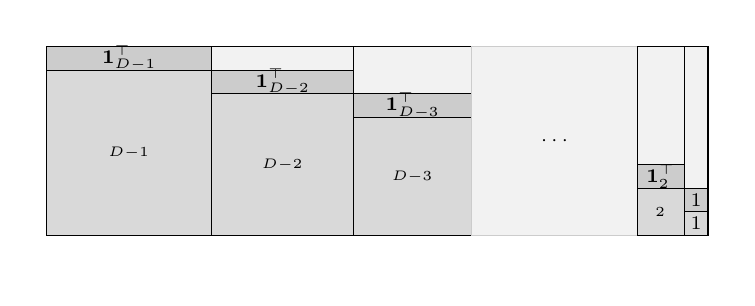
\begin{tikzpicture}[
		baseline=(current bounding box.center),
		scale=0.30,
		font=\scriptsize
	]
		\def\D{8}
		\pgfmathtruncatemacro{\Dminus}{\D*(\D-1)/2}

		% Invisible padding
		\path (-0.8,0.8) -- (\Dminus+0.8,-\D-1-0.8);

		% -------------------------------------------------
		% Start blocks: i = 1, 2, 3
		% -------------------------------------------------
		% Block 1
		\pgfmathtruncatemacro{\w}{\D-1}
		\fill[black!20] (0,0) rectangle (\w,-1);
		\draw (0,0) rectangle (\w,-1);
		\node at (\w/2,-0.5) {$\mathbf{1}_{D-1}^\top$};
		\fill[black!15] (0,-1) rectangle (\w,-\D);
		\draw (0,-1) rectangle (\w,-\D);
		\node at (\w/2,{-(1+\D)/2}) {$\I_{D-1}$};

		% Block 2
		\pgfmathtruncatemacro{\c}{\D-1}
		\pgfmathtruncatemacro{\w}{\D-2}
		\fill[black!5] (\c,0) rectangle (\c+\w,-1);
		\draw (\c,0) rectangle (\c+\w,-1);
		\fill[black!20] (\c,-1) rectangle (\c+\w,-2);
		\draw (\c,-1) rectangle (\c+\w,-2);
		\node at (\c+\w/2,-1.5) {$\mathbf{1}_{D-2}^\top$};
		\fill[black!15] (\c,-2) rectangle (\c+\w,-\D);
		\draw (\c,-2) rectangle (\c+\w,-\D);
		\node at (\c+\w/2,{-(2+\D)/2}) {$\I_{D-2}$};

		% Block 3
		\pgfmathtruncatemacro{\c}{2*\D-3}
		\pgfmathtruncatemacro{\w}{\D-3}
		\fill[black!5] (\c,0) rectangle (\c+\w,-2);
		\draw (\c,0) rectangle (\c+\w,-2);
		\fill[black!20] (\c,-2) rectangle (\c+\w,-3);
		\draw (\c,-2) rectangle (\c+\w,-3);
		\node at (\c+\w/2,-2.5) {$\mathbf{1}_{D-3}^\top$};
		\fill[black!15] (\c,-3) rectangle (\c+\w,-\D);
		\draw (\c,-3) rectangle (\c+\w,-\D);
		\node at (\c+\w/2,{-(3+\D)/2}) {$\I_{D-3}$};

		% -------------------------------------------------
		% Gap with ... (only when D > 6)
		% -------------------------------------------------
		\ifnum\D>6
			\pgfmathtruncatemacro{\gapstart}{3*\D-6}
			\pgfmathtruncatemacro{\gapend}{\Dminus-3}
			\pgfmathtruncatemacro{\gapwidth}{\gapend-\gapstart}
			\fill[black!5] (\gapstart,0) rectangle (\gapend,-\D);
			\draw[black!20] (\gapstart,0) rectangle (\gapend,-\D);
			\node at (\gapstart+\gapwidth/2,-\D/2) {$\cdots$};
		\fi

		% -------------------------------------------------
		% End blocks: i = D-2, D-1 (only when D > 6)
		% -------------------------------------------------
		\ifnum\D>6
			% Block D-2
			\pgfmathtruncatemacro{\c}{\Dminus-3}
			\pgfmathtruncatemacro{\w}{2}
			\pgfmathtruncatemacro{\zh}{\D-3}
			\fill[black!5] (\c,0) rectangle (\c+\w,-\zh);
			\draw (\c,0) rectangle (\c+\w,-\zh);
			\fill[black!20] (\c,-\zh) rectangle (\c+\w,-\zh-1);
			\draw (\c,-\zh) rectangle (\c+\w,-\zh-1);
			\node at (\c+\w/2,-\zh-0.5) {$\mathbf{1}_{2}^\top$};
			\fill[black!15] (\c,-\zh-1) rectangle (\c+\w,-\D);
			\draw (\c,-\zh-1) rectangle (\c+\w,-\D);
			\node at (\c+\w/2,{-(\zh+1+\D)/2}) {$\I_{2}$};

			% Block D-1
			\pgfmathtruncatemacro{\c}{\Dminus-1}
			\pgfmathtruncatemacro{\w}{1}
			\pgfmathtruncatemacro{\zh}{\D-2}
			\fill[black!5] (\c,0) rectangle (\c+\w,-\zh);
			\draw (\c,0) rectangle (\c+\w,-\zh);
			\fill[black!20] (\c,-\zh) rectangle (\c+\w,-\zh-1);
			\draw (\c,-\zh) rectangle (\c+\w,-\zh-1);
			\node at (\c+\w/2,-\zh-0.5) {$1$};
			\fill[black!15] (\c,-\zh-1) rectangle (\c+\w,-\D);
			\draw (\c,-\zh-1) rectangle (\c+\w,-\D);
			\node at (\c+\w/2,{-(\zh+1+\D)/2}) {$1$};
		\fi

		% % Blank zero row
		% \fill[black!0] (0,-\D) rectangle (\Dminus,-\D-1);
		% \draw (0,-\D) rectangle (\Dminus,-\D-1);

	\end{tikzpicture}}}
	\right]
\end{equation}
be the incidence matrix of the complete graph $\mathcal{G}^\ast$ with $D$ vertices. Denote $\C_{\mathcal{W}}^\top\in\{0,1\}^{D\times |\mathcal{W}|}$ as the incidence matrix of the active edges, formed by the columns of $\C^\top$ indexed by $\mathcal{W}$, and define $\Q_{11}\coloneqq\frac{2}{D}\I_D-\frac{D-2}{D^2(D-1)}\mathbf{1}_D\mathbf{1}_D^\top$. The Schur complement of $\M_{\mathcal{W}}|\P$ with respect to $\N_{11}$ is computed in Appendix~\ref{app:active_set_kkt} and given by
\begin{equation}\label{eq:S2_def_main}
	\mathbf{S}_2
	\coloneqq
	(\M_{\mathcal{W}}|\P)|\N_{11}
	=
	-\frac12\I_{|\mathcal{W}|}
	-\frac14\C_{\mathcal{W}}\Q_{11}\C_{\mathcal{W}}^\top.
\end{equation}

In an active-set method, the working set changes by adding or removing a single edge. We describe the addition update first; the removal update is the symmetric rank-1 downdate obtained by reversing the same correction.

\paragraph{Adding an edge.} When an edge $e_{k+1}$ enters the working set, $\mathcal{W}_{k+1}=\mathcal{W}_k\cup\{e_{k+1}\}$ and the matrix $\C_{\mathcal{W}_{k+1}}$ is obtained from $\C_{\mathcal{W}_k}$ by appending the row vector $\c_{k+1}^\top\in\{0,1\}^D$ associated with the new edge,
\begin{equation}
\C_{\mathcal{W}_{k+1}}^\top = \begin{bmatrix} \C_{\mathcal{W}_k}^\top & \c_{k+1}^\top \end{bmatrix},
\end{equation}
where $\c_{k+1}$ contains exactly two entries equal to $1$ (vertices at the endpoints of $e_{k+1}$) and zeros elsewhere. As shown in Appendix~\ref{app:active_set_kkt}, substituting $\C_{\mathcal{W}_{k+1}}$ into the explicit expression for $\mathbf{S}_2$ yields the bordered form
\begin{equation}
	\mathbf{S}_2^{(k+1)}
	=
	\begin{bmatrix}
		\mathbf{S}_2^{(k)} & \u_{k+1}\\
		\u_{k+1}^\top & \gamma_{k+1}
	\end{bmatrix},
\end{equation}
where the entries of $\u_{k+1}\in\R^{|\mathcal{W}|}$ depend only on whether an active edge shares a vertex with the new edge,
\begin{equation}\label{eq:u_entrywise_main}
	[\u_{k+1}]_i=
	\begin{cases}
		\displaystyle\frac{-D^2+3D-4}{2D^2(D-1)}, & e_i\sim e,\\[8pt]
		\displaystyle\frac{D-2}{D^2(D-1)}, & e_i\not\sim e,
	\end{cases}
	\qquad i=1,\dots,|\mathcal{W}|,
\end{equation}
and the scalar border is
\begin{equation}\label{eq:gamma_main}
	\gamma_{k+1}=\frac{-D^3-D^2+4D-4}{2D^2(D-1)}.
\end{equation}
Using the block-inversion formula, the inverse of the bordered matrix is obtained from $(\mathbf{S}_2^{(k)})^{-1}$ as
\begin{equation}\label{eq:S2_inv_update}
(\mathbf{S}_2^{(k+1)})^{-1} = \begin{bmatrix} (\mathbf{S}_2^{(k)})^{-1} + \frac{1}{\sigma_{k+1}}\v_{k+1}\v_{k+1}^\top & -\frac{1}{\sigma_{k+1}}\v_{k+1} \\[2pt] -\frac{1}{\sigma_{k+1}}\v_{k+1}^\top & \frac{1}{\sigma_{k+1}} \end{bmatrix},
\end{equation}
where $\v_{k+1}\coloneqq(\mathbf{S}_2^{(k)})^{-1}\u_{k+1}$ and $\sigma_{k+1}\coloneqq\gamma_{k+1}-\u_{k+1}^\top\v_{k+1}=\gamma_{k+1}-\u_{k+1}^\top(\mathbf{S}_2^{(k)})^{-1}\u_{k+1}$. Consequently $(\mathbf{S}_2^{(k)})^{-1}$ can be maintained with rank-1 updates (adding) or downdates (removing) at cost $\mathcal{O}(|\mathcal{W}|^2)$ per iteration, avoiding the $\mathcal{O}(|\mathcal{W}|^3)$ expense of recomputing the inverse from scratch. 

The $\lh_\mathcal{W}$-update uses the auxiliary vector $\z_{k+1}$, computed from the extended incidence matrix as
\begin{equation}\label{eq:z_update_main}
	\z_{k+1}
	=
	\begin{bmatrix}
		\displaystyle\frac{1}{D}(\w_{k+1}-\c_{k+1})-\frac{D-2}{D^2(D-1)}(s_{k+1}-1)\mathbf{1}_D\\[8pt]
		\displaystyle-\frac{1}{D(D-1)}(s_{k+1}-1)
	\end{bmatrix},
\end{equation}
where $\w_{k+1}\coloneqq\C_{\mathcal{W}_{k+1}}^\top\v_{k+1}$ and $s_{k+1}\coloneqq\mathbf{1}_{|\mathcal{W}_{k+1}|}^\top\v_{k+1}$ (see Appendix~\ref{app:active_set_kkt}). It also uses the residual $\r_{\mathcal{W}_{k+1}}\coloneqq\tilde{\A}_{\mathcal{W}_{k+1}}\P^{-1}\q - \tilde{\b}_{\mathcal{W}_{k+1}}$. Because the equality constraints are never modified, this residual splits into
\begin{equation}
	\r_{\mathcal{W}_{k+1}}
	\coloneqq
	\begin{bmatrix}
		\A \\ \B_{\mathcal{W}_{k+1}}
	\end{bmatrix}\P^{-1}\q -
	\begin{bmatrix}
		\b \\ \mathbf{0}
	\end{bmatrix} =
	\begin{bmatrix}
		\r_0 \\
		\r_{k+1}
	\end{bmatrix},
\end{equation}
a fixed part $\r_0\coloneqq\A\P^{-1}\q-\b$ and a working-set-related part $\r_{k+1}\coloneqq\B_{\mathcal{W}_{k+1}}\P^{-1}\q$ that is the one updated as the working set changes. Adding an edge $e_{k+1}$ to the working set is equivalent to adding a new row $\b_{k+1}$ to $\B_{\mathcal{W}_{k+1}}=[\B_{\mathcal{W}_k}^\top\ \b_{k+1}]^\top$, so the new residual vector is obtained as
\begin{equation}
	\r_{k+1}
	\coloneqq
	\begin{bmatrix}
		\r_k \\ r_{k+1}
	\end{bmatrix},
	\qquad
	r_{k+1}\coloneqq \b_{k+1}^\top\P^{-1}\q - \tilde{b}_{k+1},
\end{equation}
Define the scalar
\begin{equation}
	\label{eq:tau_update}
	\tau_{k+1}
	\coloneqq
	\begin{bmatrix}
		\z_{k+1}^\top & -\v_{k+1}^\top & 1
	\end{bmatrix}
	\r_{\mathcal{W}_{k+1}}.
\end{equation}
Finally, the dual and primal variable updates are computed in Appendix~\ref{app:active_set_kkt} and given by the rank-1 corrections
\begin{equation}
	\label{eq:nu_update}
	\boldsymbol{\nu}_{\mathcal{W}_{k+1}}
	=
	\begin{bmatrix}
		\boldsymbol{\nu}_{\mathcal{W}_k} \\ 0
	\end{bmatrix}
	+
	\frac{\tau_{k+1}}{\sigma_{k+1}}
	\begin{bmatrix}
		\z_{k+1} \\ -\v_{k+1} \\ 1
	\end{bmatrix},
\end{equation}
and
\begin{equation}
	\label{eq:lambda_from_nu}
	\lh_{\mathcal{W}_{k+1}}
	=
	\P^{-1}\q - \P^{-1}\tilde{\A}_{\mathcal{W}_{k+1}}^\top\boldsymbol{\nu}_{\mathcal{W}_{k+1}}.
\end{equation}

\paragraph{Removing an edge.} Suppose the edge at position $j\in\{1,\dots,|\mathcal{W}_k|\}$ leaves the working set, so $\mathcal{W}_{k+1}=\mathcal{W}_k\setminus\{e_j\}$. Let $\c_j\in\{0,1\}^D$ be its incidence vector and let $\C^{(k+1)}$ denote $\C_{\mathcal{W}_k}$ with row $j$ removed. As detailed in Appendix~\ref{app:active_set_kkt}, after permuting the leaving edge to the last position with a permutation matrix $\mathbf{P}_j$, the current Schur complement can be written in the bordered form
\begin{equation}
	\mathbf{P}_j\mathbf{S}_2^{(k)}\mathbf{P}_j^\top
	=
	\begin{bmatrix}
		\mathbf{S}_2^{(k+1)} & \u_{k+1}\\
		\u_{k+1}^\top & \gamma_{k+1}
	\end{bmatrix}.
\end{equation}
Equivalently, the entries of $\u_{k+1}$ are again given by~\eqref{eq:u_entrywise_main} with $e$ taken as the removed edge, and $\gamma_{k+1}$ is the same scalar as in~\eqref{eq:gamma_main}. Extract from the maintained inverse the $j$-th diagonal and off-diagonal entries,
\begin{equation}
	d_{k+1}\coloneqq[(\mathbf{S}_2^{(k)})^{-1}]_{jj},
\qquad
\tilde{\v}_{k+1}\coloneqq((\mathbf{S}_2^{(k)})^{-1})_{\setminus j,j},
\end{equation}
set $\sigma_{k+1}\coloneqq 1/d_{k+1}$ and $\v_{k+1}\coloneqq-\sigma_{k+1}\tilde{\v}_{k+1}$. The downdated inverse is then
\begin{equation}\label{eq:S2_inv_downdate_main}
	(\mathbf{S}_2^{(k+1)})^{-1}
	=
	((\mathbf{S}_2^{(k)})^{-1})_{\setminus j,\setminus j}
	-
	\sigma_{k+1}\tilde{\v}_{k+1}\tilde{\v}_{k+1}^\top.
\end{equation}
The auxiliary vector $\z_{k+1}$ is computed with the reduced incidence matrix as
\begin{equation}
	\z_{k+1}
	=
	\begin{bmatrix}
		\displaystyle\frac{1}{D}(\w_{k+1}-\c_j)-\frac{D-2}{D^2(D-1)}(s_{k+1}-1)\mathbf{1}_D\\[10pt]
		\displaystyle-\frac{1}{D(D-1)}(s_{k+1}-1)
	\end{bmatrix},
\end{equation}
where $\w_{k+1}\coloneqq(\C^{(k+1)})^\top\v_{k+1}$ and $s_{k+1}\coloneqq\mathbf{1}_{|\mathcal{W}_{k+1}|}^\top\v_{k+1}$.

When the edge at position $j$ is removed, the active residual is shortened by deleting its $j$-th entry,
\begin{equation}
	\r_{k+1} = (\r_k)_{\setminus j}.
\end{equation}
The multiplier of the leaving edge is the $(D+1+j)$-th entry of the current dual vector,
\begin{equation}
	\alpha_{k+1}\coloneqq[\boldsymbol{\nu}_{\mathcal{W}_k}]_{D+1+j}.
\end{equation}
Reversing the rank-1 correction gives the reduced dual vector
\begin{equation}\label{eq:nu_downdate_main}
	\boldsymbol{\nu}_{\mathcal{W}_{k+1}}
	=
	(\boldsymbol{\nu}_{\mathcal{W}_k})_{\setminus(D+1+j)}
	-
	\alpha_{k+1}
	\begin{bmatrix}
		\z_{k+1}\\-\v_{k+1}
	\end{bmatrix},
\end{equation}
and the primal iterate is updated as
\begin{equation}\label{eq:lambda_downdate_main}
	\lh_{\mathcal{W}_{k+1}}
	=
	\lh_{\mathcal{W}_k}
	+
	\alpha_{k+1}
	\P^{-1}
	\tilde{\A}_{\mathcal{W}_k}^\top
	\begin{bmatrix}
		\z_{k+1}\\-\v_{k+1}\\1
	\end{bmatrix}.
\end{equation}

\begin{remark}
	Instead of forming and inverting the full KKT matrix $\M_{\mathcal{W}}$ at each working-set change, which would cost $\mathcal{O}\big((D_+ + D + |\mathcal{W}|)^3\big)$ operations and $\mathcal{O}\big((D_+ + D + |\mathcal{W}|)^2\big)$ storage, the update maintains only the sparse matrices $\A$, $\B_\mathcal{W}$ and $\C_\mathcal{W}$, the inverse ${\S_2^{(k)}}^{-1}$ of size $|\mathcal{W}|\times|\mathcal{W}|$, and the vectors $\u_k$, $\v_k$, $\w_k$, $\z_k$. The sparsity of $\A$, $\B_\mathcal{W}$, and $\C_\mathcal{W}$, together with the small size of $\S_2^{(k)}$, reduces both the per-update arithmetic cost to $\mathcal{O}\big((D+|\mathcal{W}|)^2\big)$ and the overall memory footprint.
\end{remark}

\clearpage

\begin{algorithm}[H]
	\caption{Active-set KKT update when adding an edge}
	\label{alg:active_set_add_edge}
	\begin{algorithmic}[1]
		\renewcommand{\algorithmicrequire}{\textbf{Input:}}
		\renewcommand{\algorithmicensure}{\textbf{Output:}}
		\Require Working set $\mathcal{W}$; maintained inverse $\mathbf{S}_2^{-1}$; current iterate $(\lh,\boldsymbol{\nu})$; constant residual $\r_1$; active residual $\r_2$; stacked constraint matrix $\tilde{\A}$; new edge index $i$, incidence $\c$, and constraint row $\tilde{\a}^\top$; problem data $\P$, $\q$.
		\Ensure Updated $\mathcal{W}$, $\C$, $\mathbf{S}_2^{-1}$, $\lh$, $\boldsymbol{\nu}$, $\r_2$, $\tilde{\A}$.
		\State $\g\gets\P^{-1}\q$
		\State Form $\C\in\{0,1\}^{|\mathcal{W}|\times D}$ whose rows are the incidence vectors $\{\c_j^\top\}_{j\in\mathcal{W}}$
		\State Form $\u\in\mathbb{R}^{|\mathcal{W}|}$ with
		\Statex \quad $[\u]_\ell=\frac{-D^2+3D-4}{2D^2(D-1)}$ if the $\ell$-th edge of $\mathcal{W}$ is adjacent to edge $i$, otherwise $[\u]_\ell=\frac{D-2}{D^2(D-1)}$
		\State $\gamma\gets\frac{-D^3-D^2+4D-4}{2D^2(D-1)}$
		\State $\v\gets\mathbf{S}_2^{-1}\u$
		\State $\sigma\gets\gamma-\u^\top\v$
		\State $\mathbf{S}_2^{-1}\gets\begin{bmatrix}\mathbf{S}_2^{-1}+\frac{1}{\sigma}\v\v^\top & -\frac{1}{\sigma}\v\\ -\frac{1}{\sigma}\v^\top & \frac{1}{\sigma}\end{bmatrix}$
		\State $\w\gets\C^\top\v$,\quad $s\gets\mathbf{1}_{|\mathcal{W}|}^\top\v$
		\State $\z\gets\begin{bmatrix}\frac{1}{D}(\w-\c)-\frac{D-2}{D^2(D-1)}(s-1)\mathbf{1}_D\\ -\frac{1}{D(D-1)}(s-1)\end{bmatrix}$
		\State $r\gets\tilde{\a}^\top\g$
		\State $\tau\gets\z^\top\r_1-\v^\top\r_2+r$
		\State $\boldsymbol{\nu}\gets\begin{bmatrix}\boldsymbol{\nu}\\0\end{bmatrix}+\frac{\tau}{\sigma}\begin{bmatrix}\z\\-\v\\1\end{bmatrix}$
		\State $\lh\gets\lh-\frac{\tau}{\sigma}\P^{-1}\tilde{\A}^\top\begin{bmatrix}\z\\-\v\\1\end{bmatrix}$
		\State $\r_2\gets\begin{bmatrix}\r_2\\r\end{bmatrix}$
		\State $\mathcal{W}\gets\mathcal{W}\cup\{i\}$
		\State Append $\c^\top$ to $\C$ and $\tilde{\a}^\top$ to $\tilde{\A}$
	\end{algorithmic}
\end{algorithm}

\begin{algorithm}[H]
	\caption{Active-set KKT update when removing the edge at position $j$}
	\label{alg:active_set_remove_edge}
	\begin{algorithmic}[1]
		\renewcommand{\algorithmicrequire}{\textbf{Input:}}
		\renewcommand{\algorithmicensure}{\textbf{Output:}}
		\Require Active edge list $\C$; maintained inverse $\mathbf{S}_2^{-1}$; current iterate $(\lh,\boldsymbol{\nu})$; active residual $\r_2$; stacked constraint matrix $\tilde{\A}$; position $j\in\{1,\dots,|\mathcal{W}|\}$; problem data $\P$.
		\Ensure Updated $\C$, $\mathbf{S}_2^{-1}$, $\lh$, $\boldsymbol{\nu}$, $\r_2$, $\tilde{\A}$.
		\State $m\gets|\mathcal{W}|$
		\State $\c\gets$ incidence vector of the edge at position $j$ (the $j$-th column of $\C^\top$)
		\State $d\gets[\mathbf{S}_2^{-1}]_{jj}$,\quad $\tilde{\v}\gets(\mathbf{S}_2^{-1})_{\setminus j,j}$
		\State $\sigma\gets 1/d$,\quad $\v\gets-\sigma\tilde{\v}$
		\State $\mathbf{S}_2^{-1}\gets(\mathbf{S}_2^{-1})_{\setminus j,\setminus j}-\sigma\tilde{\v}\tilde{\v}^\top$
		\State $\C_{\text{red}}\gets\C$ with row $j$ removed
		\State $\w\gets\C_{\text{red}}^\top\v$,\quad $s\gets\mathbf{1}_{m-1}^\top\v$
		\State $\z\gets\begin{bmatrix}\frac{1}{D}(\w-\c)-\frac{D-2}{D^2(D-1)}(s-1)\mathbf{1}_D\\ -\frac{1}{D(D-1)}(s-1)\end{bmatrix}$
		\State $\alpha\gets[\boldsymbol{\nu}]_{D+1+j}$\Comment{Multiplier of the removed edge}
		\State $\boldsymbol{\nu}\gets\boldsymbol{\nu}_{\setminus(D+1+j)}-\alpha\begin{bmatrix}\z\\-\v\end{bmatrix}$
		\State $\lh\gets\lh+\alpha\P^{-1}\tilde{\A}^\top\begin{bmatrix}\z\\-\v\\1\end{bmatrix}$
		\State $\r_2\gets(\r_2)_{\setminus j}$
		\State Delete row $j$ of $\C$ and row $D+1+j$ of $\tilde{\A}$
	\end{algorithmic}
\end{algorithm}

\subsection{Convergence analysis}
\label{sec:as_conv_analysis}

Under Assumptions~\ref{ass:ipm_strict_feas}--\ref{ass:ipm_pd}, the dual active-set method enjoys the following properties~\cite[\S16.5]{nocedal2006numerical}:
\begin{itemize}
	\item \emph{Finite termination.} The algorithm terminates in a finite number of iterations, bounded in the worst case by $\binom{D_-}{|\mathcal{W}_\ast|}$, but typically of order $\mathcal{O}(D_-)$ in practice.
	\item \emph{Monotonic objective decrease.} The objective $f(\lh_\mathcal{W})$ decreases monotonically as constraints are added; consequently, no working set is visited twice and cycling is precluded.
	\item \emph{No tolerance trade-off.} Unlike IPM, the active-set method terminates exactly when the KKT conditions hold and returns the optimal solution to floating-point precision, with no accuracy parameter to tune.
\end{itemize}
The total cost is $\mathcal{O}(K_\text{AS}\cdot (D+|\mathcal{W}|_{\max})^2)$, where $K_\text{AS}$ is the number of active-set updates. For sparse target graphs, $|\mathcal{W}|_{\max}\approx D_-=\mathcal{O}(D^2)$, but $K_\text{AS}$ is typically much smaller than the IPM iteration count when the algorithm is warm-started from a previous estimate of $\mathcal{W}_\ast$. Active-set methods are therefore particularly attractive in iterative graph-learning contexts where the support of the graph evolves slowly between consecutive outer iterations.

\section{Alternating direction method of multipliers}

The alternating direction method of multipliers (ADMM)~\cite{admm} is a first-order optimization algorithm designed to solve convex problems with separable objective functions and linear constraints by combining ideas from dual decomposition and augmented Lagrangian methods. ADMM proceeds by alternating simple minimization steps with respect to each variable block, followed by a dual update, which allows the problem to be decomposed into smaller and often closed-form subproblems. Although ADMM typically converges more slowly in terms of iteration count, its modest memory requirements, ease of implementation, and ability to exploit problem structure make it particularly attractive when interior point methods become computationally prohibitive.

First, define the convex set $\mathcal{D} \coloneqq \{\z\in\R^{D(D+1)/2}:\ \B\z\leq \mathbf{0}\}$ of half-vectorization vectors where the components related to the off-diagonal entries are non-positive. Then, the quadratic program in \eqref{eq:vech_lap} is reformulated using an additional variable $\z$ that is constrained to belong to $\mathcal{D}$, and adding an additional constraint so that $\z=\lh$. Therefore, the equivalent problem is expressed as
\begin{equation}
	\label{eq:lap_est_k_qp_admm} 
	\{\hat{\lh},\hat{\z}\} =\argmin_{\lh,\z\in\R^{D(D+1)/2}} \frac{1}{2}\lh^\top\P\lh - \q^\top\lh + \mathbb{I}_{\mathcal{D}}(\z) 
	\quad\text{s. t. }\ \A\lh = \b,\ \lh = \z
\end{equation}
where $\mathbb{I}_{\mathcal{D}}(\z)$ is an indicator function whose value is 0 if $\z\in\mathcal{D}$ and $+\infty$ otherwise. For the problem in \eqref{eq:lap_est_k_qp_admm}, the ADMM steps are given by
\begin{align}
	\lh_{t+1} &= \argmin_{\lh\in\R^{D(D+1)/2}} \frac{1}{2}\lh^\top\P\lh - \q^\top\lh + \frac{\rho}{2}\norm{\lh-\z_t-\v_t}^2\quad \text{s. t. }\ \A\lh = \c \label{eq:inner_admm1} \\
	\z_{t+1} &= \Pi_{\mathcal{D}}(\lh_{t+1}-\v_t) \label{eq:inner_admm2} \\
	\v_{t+1} &= \v_t + \z_{t+1} - \lh_{t+1} \label{eq:inner_admm3}
\end{align}
where $t\in\{0,1,\ldots\}$ denotes the ADMM iteration, $\rho>0$ is a quadratic regularization factor and $\Pi_{\mathcal{D}}$ is the projection operator onto the set $\mathcal{D}$. The Krush-Kuhn-Tucker (KKT) system for \eqref{eq:inner_admm1} is given by
\begin{equation}\label{eq:kkt_system_admm1}
	\M
	\left[
	\begin{array}{c}
		\lh_{t+1} \\
		\boldsymbol{\mu}_{t+1}
	\end{array}
	\right] = 
	\left[
	\begin{array}{c}
		\r_t \\
		\b
	\end{array}
	\right],\quad \text{where}\quad \M\coloneqq \left[
	\begin{array}{cll}
		\P + \rho\I & \A^\top \\
		\A & \mathbf{0}
	\end{array}
	\right],
\end{equation}
$\r_t\coloneqq \rho(\z_t+\v_t) + \q$, and
$\boldsymbol{\mu}_{t+1}\in\R^{D+1}$ is the dual variable of Lagrange multipliers. A brute force approach to solve this system would be to invert $\M$. However, here we leverage the structure of this matrix to perform a more efficient computation of the solution. Define $\Rm\coloneqq\P+\rho\I$. The Schur complement of $\M$ w.r.t. $\Rm$ is given by
\begin{equation}
	\M|\Rm = -\A\Rm^{-1}\A^\top
\end{equation}
and the inverse of $\M$ can be expressed in terms of $\M|\Rm$ as
\begin{small}
	\begin{equation}\label{eq:Minv_admm}
		\M^{-1} = \left[
		\begin{array}{cc}
			\Rm^{-1} - \Rm^{-1}\A^\top\S  & \S^\top \\
			\S & (\M|\Rm)^{-1}
		\end{array}
		\right]
	\end{equation}
\end{small}%
where $\S\coloneqq -(\M|\Rm)^{-1}\A\Rm^{-1}$. Since $\lh^\top \P \lh= \l^\top \l = \norm{\L}_F^2$, it is not difficult to check that matrix $\Rm$ is diagonal and its elements have the following structure
\begin{equation}
	\Rm=\text{diag}(1+\rho, \underbrace{2+\rho,\ldots,2+\rho}_{D-1},1+\rho, \label{eq:R} 
	\underbrace{2+\rho,\ldots,2+\rho}_{D-2},1+\rho,\ldots,1+\rho,2+\rho,1+\rho) 
\end{equation}
As a result, the Schur complement is given by
\begin{align*}
	\M|\Rm &= -\frac{1}{1+\rho}\left[
	\begin{array}{cc}
		\T  & \mathbf{1}_D \\
		\mathbf{1}_D^\top & D
	\end{array}
	\right]\quad \text{where}\quad
	\T = \left(\frac{1+\rho}{2+\rho}(D-2)+1\right)\I_D + \frac{1+\rho}{2+\rho}\mathbf{1}_D\mathbf{1}_D^\top.
\end{align*}
Notice that $\M|\Rm$ is a block matrix and the Schur complement can be leveraged again to invert it
\begin{equation*}
	(\M|\Rm)^{-1} = -(1+\rho)\left[
	\begin{array}{cc}
		\T^{-1} + \frac{1}{s}\t\t^\top  & -\frac{1}{s}\t \\
		-\frac{1}{s}\t^\top & \frac{1}{s}
	\end{array}
	\right]
\end{equation*}
where $s\coloneqq D-\mathbf{1}_D^\top\T^{-1}\mathbf{1}_D$ and $\t\coloneqq \T^{-1}\mathbf{1}_D$. Matrix $\T$ is the sum of a multiple of the identity plus a rank-one matrix, and therefore, Sherman-Morrison lemma can be leveraged to compute the inverse efficiently
\begin{align}
	&\T^{-1} = \delta_1\I_D - \delta_2\boldsymbol{1}_D\boldsymbol{1}_D^\top\label{eq:Mschur_inv} 
\end{align}
where $\delta_1\coloneqq \frac{2+\rho}{D(\rho+1)-\rho}$ and $\delta_2\coloneqq \frac{(1+\rho)\delta_1}{2D(1+\rho)-\rho}$. Therefore, $s = D-\mathbf{1}_D^\top\T^{-1}\mathbf{1}_D = (1 - \delta_1)D + \delta_2 D^2$, and $\t=\delta_3\mathbf{1}_D$, where $\delta_3\coloneqq \delta_1-\delta_2D$. Replacing~\eqref{eq:Mschur_inv} back in~\eqref{eq:Minv_admm} and using~\eqref{eq:kkt_system_admm1} yields
\begin{equation*}
	\lh_{t+1} = \Rm^{-1}\r_t - \Rm^{-1}\A^\top\S\r_t + \S^\top\b = 
	\Rm^{-1}(\r_t + \A^\top(\M|\Rm)^{-1}\s_t)
\end{equation*}
where $\s_t\coloneqq \A\Rm^{-1}\r_t-\b$. Now, split matrix $\A$ as $\A=[\A_1^\top \a_2]^\top$, where $\A_1\in\{0,1\}^{D\times D_+}$ denotes the sub-block containing the first $D$ rows of $\A$, and $\a_2\in\{0,1\}^{D_+}$ denotes the last row of $\A$. Similarly, split vector $\s_t=[\s_{t,1}^\top, s_{t,2}]^\top$, where $\s_{t,1}\in\R^D$ and $s_{t,2}\in\R$. Then, we have 
\begin{small}
	\begin{align*}
		\A^\top(\M|\Rm)^{-1}\s_t = -(1+\rho)(\delta_1\A_1^\top\s_{t,1} + \nu_{1,t}\th + \nu_{2,t}\a_2)
	\end{align*}
\end{small}%
where the constants $\nu_{1,t}\coloneqq s^{-1}\delta_3(\delta_3\xi_t-s_{t,2}) - \delta_2\xi_t$ and $\nu_{2,t}\coloneqq s^{-1}(s_{t,2} - \delta_3\xi_t)$; and where $\xi_t\coloneqq \mathbf{1}_D^\top\s_{t,1}$, and
\begin{equation*}
	\th\coloneqq\A_1^\top\mathbf{1}_D = [1, \underbrace{2,\ldots,2}_{D-1},1,\underbrace{2,\ldots,2}_{D-2},1,\ldots,1,2,1]^\top.
\end{equation*}
Note that $\lh_{t+1}$ can be efficiently computed since $\Rm^{-1}$ is a diagonal matrix and $\A$ is a sparse matrix. 

The next step of the algorithm is the projection onto $\mathcal{D}$ given by~\eqref{eq:inner_admm2}. Define $\w_t\coloneqq \lh_{t+1}-\v_t$. Then, \eqref{eq:inner_admm2} can be expressed as
\begin{equation}\label{eq:z_problem}
	\z_{t+1} = \argmin_{\boldsymbol{\z}\in\R^{D(D+1)/2}} \frac{1}{2}\norm{\z-\w_t}_2^2\quad  \text{s. t.}\quad
	\B\z\leq \mathbf{0}
\end{equation}
\noindent which is a projection onto the non-positive orthant whose solution is given by $\z_{t+1} = \w_t - \B^\top\B\max(\w_t,\mathbf{0})$. \\

\noindent \textbf{Remark}: vectors $\z_t$, $\v_t$ and $\q$ have length $D_+$, and $\Rm^{-1}$ is a $D_+\times D_+$ diagonal matrix. Therefore, computing $\r_t$ and $\Rm^{-1}\r_t$  requires $\mathcal{O}(D_+)$ operations and $\mathcal{O}(D_+)$ storage. Matrix $\A\in\{0,1\}^{(D+1)\times D_+}$ contains 2 non-zero elements in each column and therefore, the products $\A\Rm^{-1}\r_t$ requires $\mathcal{O}(D+1)$ operations. Finally, computing $\A_1^\top\boldsymbol{1}_D$ and $\A_1^\top\s_t$ requires $\mathcal{O}(D)$ operations. The rest of operations are scalar operations that are computationally negligible. As a result, computing $\lh_{t+1}$ requires $\mathcal{O}(D_+)$ operations, whereas naive inversion of $\M^{-1}$ would cost $\mathcal{O}((D_++D+1)^3)$ operations.

\begin{algorithm}[t]
	\caption{Laplacian Projection via ADMM}
	\label{alg:ladmm}
	\begin{algorithmic}[1]
		\renewcommand{\algorithmicrequire}{\textbf{Input:}}
		\renewcommand{\algorithmicensure}{\textbf{Output:}}
		\Require Matrix to project $\boldsymbol{\Gamma}\in\R^{D\times D}$; equality constraint matrix $\A\in\{0,1\}^{(D+1)\times D_+}$; equality constraint vector $\b\in\{0,V\}^{D+1}$; inequality constraint matrix $\B\in\{0,1\}^{D_-\times D_+}$; duplication matrix $\J\in\{0,1\}^{D_+\times D^2}$; Lagrangian term $\rho>0$; tolerance $\epsilon >0$; maximum number of iterations $T$.
		\Ensure Projected Laplacian matrix $\L\in\mathcal{L}$.
		\State $\lh\gets \mathbf{0}$, $\z\gets \mathbf{0}$, $\v\gets\mathbf{0}$
		\State $\q\gets \J\text{vec}(\boldsymbol{\Gamma})$
		\State $\A_1\gets [\A]_{1:D}$,\ $\a_2\gets[\A]_{D+1}$
		\State Build $\Rm$ as in~\eqref{eq:R}
		\State $t\gets 0$, $e\gets \epsilon + 1$
		\While{$e>\epsilon$ \textbf{ and } $t < T$}
		\State $\lh_{\text{old}}\gets \lh$
		\State $\r\gets \Rm^{-1}(\rho(\z+\v) + \q)$
		\State $\s\gets \A\Rm^{-1}\r-\b$,\ $\s_1\gets [\s]_{1:D}$,\ $s_2\gets [\s]_{D+1}$
		\State $\delta_1\gets \frac{2+\rho}{D(\rho+1)-\rho}$,\ $\delta_2\gets \frac{(1+\rho)\delta_1}{2D(1+\rho)-\rho}$,\ $\delta_3\gets \delta_1-\delta_2D$
		\State $s \gets (1 - \delta_1)D + \delta_2 D^2$
		\State $\xi\gets \mathbf{1}_D^\top\s_1$
		\State $\nu_{1}\gets s^{-1}\delta_3(\delta_3\xi-s_2) - \delta_2\xi$
		\State $\nu_{2}\gets s^{-1}(s_2 - \delta_3\xi)$
		\State $\th\gets\A_1^\top\mathbf{1}_D$
		\State $\t \gets -(1+\rho)(\delta_1\A_1^\top\s_1 + \nu_1\th + \nu_2\a_2)$
		\State $\lh\gets \Rm^{-1}(\r+\t)$
		\State $\w\gets\lh - \v$
		\State $\z \gets \w - \B^\top\B\max(\w,\mathbf{0})$
		\State $\v \gets \v + \z - \lh$
		\State $e\gets \norm{\lh-\lh_{\text{old}}}$
		\State $t \gets t + 1$
		\EndWhile
		\State $\L \gets \text{vech}^{-1}(\lh)$
		\Return $\L$ 
	\end{algorithmic} 
\end{algorithm}

\subsection{Convergence analysis}
\label{sec:conv_analysis}

ADMM converges to a solution if the problem is feasible in~\cite{admm}. However, the convergence rate and the optimal step size $\rho_\ast$ are problem-dependent and have to be studied independently. The family of quadratic programs to which \eqref{eq:vech_lap} belongs is studied in~\cite{optimal_step}. First, define $D_+\coloneqq D(D+1)/2$ and $D_-\coloneqq D(D-1)/2$. The matrix $\A\in\{0,1\}^{D\times D_+}$ has $\text{rank}(\A)=D$. Therefore, its column nullspace is spanned by an orthonormal base of $D_-$ vectors represented by the columns of the basis matrix $\N\in\R^{D_+\times D_-}$ such that $\A\N=\mathbf{0}$. The convergence analysis in~\cite{optimal_step} relies on the following assumptions.  
\begin{assumption}\label{assumption1}
	The quadratic program in~\eqref{eq:vech_lap} is feasible, i.e., there exists $\lh_\ast\in\mathcal{D}$ such that $\A\lh_\ast=\mathbf{0}$.
\end{assumption}
\begin{assumption}\label{assumption2}
	Matrix $\A$ has full row rank $D$.
\end{assumption}
\begin{assumption}\label{assumption3}
	The Hessian is positive definite on the column nullspace of $\A$, i.e., $\tilde\P\coloneqq\N^\top\P\N\succ\mathbf{0}$.
\end{assumption}
\noindent The constraints in Assumption~\ref{assumption1} in matrix form are Laplacian matrix constraints and since $\mathcal{L}$ is non-empty, Assumption~\ref{assumption1} holds. Also, the rows of $\A\in\{0,1\}^{D\times D_+}$ are linearly independent by construction and Assumption~\ref{assumption2} holds. Finally, we have the following lemma.
\begin{lemma}
	The eigenvalues of $\tilde\P$ are bounded by
	\begin{equation}\label{eq:bounds_lambda_P}
		\lambda_{\min}(\P) \leq \lambda_i(\tilde\P) \leq \lambda_{\max}(\P)
	\end{equation}
	for $i=0,\ldots,D_--1$.
	\begin{proof}
		Denote by $R(\M,\x) \coloneqq \frac{\x^\top\M\x}{\x^\top\x}$ the Rayleigh quotient of a real symmetric matrix $\M\in\R^{m\times m}$ and vector $\x\in\R^m$. Note that, $\forall \x\in\R^{D_-}$
		\begin{equation*}
			R(\tilde\P,\x) = \frac{\x^\top\tilde\P\x}{\x^\top\x} = \frac{\x^\top\N^\top\P\N\x}{\x^\top\N^\top\N\x} = R(\P,\N\x)
		\end{equation*}
		because $\N^\top\N=\I$. Therefore, the $i^\text{th}$ eigenvalue of $\tilde{\P}$ is equal to $\lambda_i(\tilde{\P})=R(\tilde\P,\v_i)=R(\P,\N\v_i)$, where $\v_i$ the $i^\text{th}$ eigenvector of $\tilde{\P}$. Since 
		\begin{equation*}
			\lambda_{\min}(\P) \leq R(\P,\N\v_i) \leq \lambda_{\max}(\P),
		\end{equation*}
		then~\eqref{eq:bounds_lambda_P} holds. 
	\end{proof}
\end{lemma}
\noindent Since $\P\succ\mathbf{0}$ is diagonal, $\lambda_{\min}(\P)=1>0$, and Assumption~\ref{assumption3} is true.

Under Assumptions~\ref{assumption1}-\ref{assumption3}, the following theorems from~\cite{optimal_step} provide the main convergence results for the quadratic program in~\eqref{eq:vech_lap}.

\begin{theorem}[Corollary 1, \cite{optimal_step}]
	Suppose Assumptions~\ref{assumption1}-\ref{assumption3} hold and $\rho>0$. Then, (i) $\{(\z_t,\u_t)\}_{t\geq1}$ converges $R$-linearly to $\{(\z_\ast,\u_\ast)\}$ and (ii) $\{(\z_t,\u_t)\}_{t\geq2}$ converges 2-step $Q$-linearly to $\{(\z_\ast,\u_\ast)\}$.
\end{theorem}

\begin{theorem}[Theorem 4, \cite{optimal_step}]
	Suppose Assumptions~\ref{assumption1}-\ref{assumption3} hold and $\rho>0$. Then, the optimal step-size is given by
	\begin{equation*}
		\rho_\ast=\sqrt{\lambda_{\min}(\tilde{\P})\lambda_{\max}(\tilde{\P})}.
	\end{equation*}	
\end{theorem}%
\noindent The values of $\lambda_{\min}(\tilde{\P})$ and $\lambda_{\max}(\tilde{\P})$ require computing the nullspace matrix $\N$. However, using the bounds on~\eqref{eq:bounds_lambda_P}, we can provide a range on which the optimal step size lies, which is given by $\rho\in[1,2]$.

Algorithm~\ref{alg:ladmm} summarizes the described ALP iteration to solve problem~\eqref{eq:vech_lap}, Algorithm~\ref{alg:outer_admm} the outer ADMM iteration to compute the Laplacian update, and Algorithm~\ref{alg:precision_palm} the overall pseudocode for the PALM updates particularized to the graph learning problem in~\eqref{eq:MAP_restrict_form}, that we named Polynomial Autoregressive (POLAR) graph learning.


% \section{Homogeneous self-dual embedding}
% \label{sec:hsde}

% The homogeneous self-dual embedding (HSDE) is a unified framework that reformulates a convex optimization problem together with its dual and the associated optimality conditions into a single feasibility problem. By embedding the primal--dual pair into a higher-dimensional homogeneous system, HSDE enables the simultaneous detection of optimality, primal infeasibility, or dual infeasibility within the same algorithmic structure. When solved with operator-splitting methods, the homogeneous formulation yields a parameter-free algorithm that does not require tuning penalty parameters or step sizes. Compared with ADMM, whose convergence can be sensitive to the penalty parameter, HSDE offers increased robustness and ease of use, while retaining scalability for large-scale conic programs.

% \begin{definition}[Cone and dual cone]
% 	A set $\mathcal{K}\subseteq\R^n$ is a \emph{cone} if $\theta\x\in\mathcal{K}$ for every $\x\in\mathcal{K}$ and every $\theta\geq 0$; it is a \emph{convex cone} if it is both a cone and a convex set. The \emph{dual cone} of $\mathcal{K}$ is
% 	\begin{equation}
% 		\mathcal{K}_*\coloneqq\{\z\in\R^n:\z^\top\x\geq 0\ \text{for all}\ \x\in\mathcal{K}\}.
% 	\end{equation}
% \end{definition}

% Conic constraints generalize linear inequality constraints: for example, $\x\geq\mathbf{0}$ is the requirement that $\x$ lie in the nonnegative orthant cone. We start again from the QP in~\eqref{eq:lap_est_qp},
% \begin{equation}
% 	\hat{\lh} = \argmin_{\lh\in\R^{D_+}} \frac{1}{2}\lh^\top\P\lh - \q^\top\lh\quad \text{s. t.}\ \A\lh = \b,\ \B\lh \leq \mathbf{0}.
% \end{equation}
% HSDE requires a linear objective with conic constraints, so the quadratic term is first epigraphized. Introduce $t\in\R$ such that
% \begin{equation}
% 	t \geq \frac{1}{2}\lh^\top\P\lh.
% \end{equation}
% Using $\P=\beta\D^\top\D$, this is equivalent to
% \begin{equation}
% 	\norm{\sqrt{\beta}\D\lh}^2 \leq 2t,
% \end{equation}
% which is a rotated second-order cone (rSOC) constraint on $[\sqrt{\beta}\D\lh^\top, t, 2]^\top$. Introducing a slack vector $\s\in\R_+^{D_-}$ for the inequality constraints through $\B\lh+\s=\mathbf{0}$, the QP becomes the conic linear program
% \begin{equation}\label{eq:hsde_conic_lp}
% 	\min_{\lh,t,\s}\ t - \q^\top\lh \quad\text{s. t.}\quad \A\lh=\b,\ \B\lh+\s=\mathbf{0},\ \s\geq\mathbf{0},\ [\sqrt{\beta}\D\lh^\top,t,2]^\top\in\mathcal{Q}_r,
% \end{equation}
% where $\mathcal{Q}_r\subset\R^{D^2+2}$ denotes the rotated second-order cone
% \begin{equation}
% 	\mathcal{Q}_r \coloneqq \left\{[\y^\top,u,v]^\top\in\R^{D^2+2}:\ \norm{\y}^2\leq uv,\ u\geq 0,\ v\geq 0\right\}.
% \end{equation}

% To write~\eqref{eq:hsde_conic_lp} in the standard conic form, it is convenient to treat the constant $v=2$ as an auxiliary variable fixed by an equality constraint. Stack the variables as
% \begin{equation}
% 	\x \coloneqq [\lh^\top,\ t,\ \s^\top,\ v]^\top \in\R^{N_x},\quad N_x\coloneqq D_+ + D_- + 2,
% \end{equation}
% and define
% \begin{equation}
% 	\A_0 \coloneqq \begin{bmatrix}\A & \mathbf{0}_{(D+1)\times 1} & \mathbf{0}_{(D+1)\times D_-} & \mathbf{0}_{D+1}\\ \B & \mathbf{0}_{D_-\times 1} & \I_{D_-} & \mathbf{0}_{D_-}\\ \mathbf{0}_{D_+}^\top & 0 & \mathbf{0}_{D_-}^\top & 1\end{bmatrix}\in\R^{m\times N_x},\quad
% 	\b_0 \coloneqq \begin{bmatrix}\b\\ \mathbf{0}_{D_-}\\ 2\end{bmatrix}\in\R^m,
% \end{equation}
% with $m\coloneqq D+D_-+2$, and
% \begin{equation}
% 	\c \coloneqq [-\q^\top,\ 1,\ \mathbf{0}_{D_-}^\top,\ 0]^\top\in\R^{N_x}.
% \end{equation}
% The closed convex cone is
% \begin{equation}
% 	\mathcal{K} \coloneqq \left\{[\lh^\top,t,\s^\top,v]^\top\in\R^{N_x}:\ [\sqrt{\beta}\D\lh^\top,t,v]^\top\in\mathcal{Q}_r,\ \s\geq\mathbf{0}\right\}=\mathcal{Q}_r\times\R_+^{D_-}.
% \end{equation}
% Problem~\eqref{eq:hsde_conic_lp} then reads
% \begin{equation}\label{eq:hsde_standard}
% 	\min_{\x}\ \c^\top\x \quad\text{s. t.}\quad \A_0\x=\b_0,\ \x\in\mathcal{K}.
% \end{equation}

% The dual is derived from the Lagrangian of~\eqref{eq:hsde_standard},
% \begin{equation}
% 	\mathcal{L}(\x,\y)=\c^\top\x + \y^\top(\A_0\x-\b_0) + \mathbb{I}_{\mathcal{K}}(\x)
% 	= -\b_0^\top\y + (\c+\A_0^\top\y)^\top\x + \mathbb{I}_{\mathcal{K}}(\x),
% \end{equation}
% where $\mathbb{I}_{\mathcal{K}}$ denotes the indicator function of $\mathcal{K}$. The dual function is
% \begin{equation}
% 	g(\y)=\inf_{\x}\mathcal{L}(\x,\y)
% 	= -\b_0^\top\y + \inf_{\x\in\mathcal{K}}(\c+\A_0^\top\y)^\top\x.
% \end{equation}
% Since $\mathcal{K}$ is a cone, the inner infimum is $0$ when $\c+\A_0^\top\y\in\mathcal{K}_*$ (because then $(\c+\A_0^\top\y)^\top\x\geq 0$ for every $\x\in\mathcal{K}$, with equality at $\x=\mathbf{0}$), and $-\infty$ otherwise. Therefore, the dual of~\eqref{eq:hsde_standard} is
% \begin{equation}
% 	\max_{\y}\ -\b_0^\top\y \quad\text{s. t.}\quad \c+\A_0^\top\y\in\mathcal{K}_*,
% \end{equation}
% where $\mathcal{K}_*$ is the dual cone of $\mathcal{K}$. Strong duality holds because Slater's condition is satisfied for the original QP. The KKT conditions are
% \begin{equation}
% 	\A_0\x^*=\b_0,\quad \x^*\in\mathcal{K},\quad \r^*\coloneqq\c+\A_0^\top\y^*\in\mathcal{K}_*,\quad \c^\top\x^*+\b_0^\top\y^*=0,
% \end{equation}
% where the first two requirements are \emph{primal feasibility}, the third is \emph{dual feasibility} (the dual variable must lie in the dual cone), and the last equality is the \emph{zero-duality-gap} condition. To see why the gap takes this form, combine the primal objective $\c^\top\x^*$ with the dual objective $-\b_0^\top\y^*$. Under strong duality the optimal values coincide, so $\c^\top\x^*=-\b_0^\top\y^*$, which is exactly $\c^\top\x^*+\b_0^\top\y^*=0$. Equivalently, this last condition encodes \emph{complementary slackness}: because $\r^*\in\mathcal{K}_*$ and $\x^*\in\mathcal{K}$, we have $(\r^*)^\top\x^*\geq 0$; substituting $\r^*=\c+\A_0^\top\y^*$ and using $\A_0\x^*=\b_0$ gives $(\r^*)^\top\x^*=\c^\top\x^*+\b_0^\top\y^*$, so zero duality gap is the same as $(\r^*)^\top\x^*=0$. The homogeneous self-dual embedding introduces a nonnegative scaling pair $(\tau,\kappa)$ and combines these conditions into the single linear system
% \begin{equation}\label{eq:hsde_system}
% 	\begin{bmatrix}\r\\ \mathbf{0}\\ \kappa\end{bmatrix}
% 	=
% 	\begin{bmatrix}
% 		\mathbf{0} & \A_0^\top & \c\\
% 		-\A_0 & \mathbf{0} & \b_0\\
% 		-\c^\top & -\b_0^\top & 0
% 	\end{bmatrix}
% 	\begin{bmatrix}\x\\ \y\\ \tau\end{bmatrix}
% 	=
% 	\Q
% 	\begin{bmatrix}\x\\ \y\\ \tau\end{bmatrix},
% \end{equation}
% with the conic membership constraints
% \begin{equation}\label{eq:hsde_cones}
% 	(\x,\tau)\in\mathcal{K}\times\R_+,\qquad (\r,\kappa)\in\mathcal{K}_*\times\R_+.
% \end{equation}
% We denote the combined variable by $\v\coloneqq[\x^\top,\y^\top,\tau]^\top$ and the cone by $\mathcal{C}\coloneqq\mathcal{K}\times\R^m\times\R_+$. The HSDE feasibility problem is then
% \begin{equation}\label{eq:hsde_feas}
% 	\text{find }\v\quad\text{s. t.}\quad \Q\v\in\mathcal{C}_*,\ \v\in\mathcal{C},
% \end{equation}
% where $\mathcal{C}_*\coloneqq\mathcal{K}_*\times\{\mathbf{0}\}\times\R_+$ is the dual cone of $\mathcal{C}$.

% The possible values of $(\tau,\kappa)$ characterize the outcome~\cite{conic}:
% \begin{enumerate}
% 	\item $\tau>0$, $\kappa=0$: the point $(\hat{\x},\hat{\y})=(\x^*/\tau,\y^*/\tau)$ satisfies the KKT conditions and is a primal--dual solution.
% 	\item $\tau=0$, $\kappa>0$: the duality gap is negative, which means the original problem is primal or dual infeasible.
% 	\item $\tau=\kappa=0$: if either $\c^\top\x<0$ or $\b_0^\top\y<0$, the problem is infeasible; otherwise no conclusion can be drawn.
% \end{enumerate}

% Problem~\eqref{eq:hsde_feas} can be solved by the three-operator splitting of~\cite{conic}, which reduces to the simple ADMM-like iteration
% \begin{align}
% 	\tilde{\v}_{n+1} &= (\I+\Q)^{-1}(\v_n+\w_n),\label{eq:hsde_admm1}\\
% 	\v_{n+1} &= \Pi_{\mathcal{C}}(\tilde{\v}_{n+1}-\w_n),\label{eq:hsde_admm2}\\
% 	\w_{n+1} &= \w_n - \tilde{\v}_{n+1} + \v_{n+1}.\label{eq:hsde_admm3}
% \end{align}
% The algorithm is parameter-free: no step-size or penalty tuning is required beyond the convergence tolerance.

% \subsection{Linear system solution}

% The first step of the iteration is the solution of the sparse linear system
% \begin{equation}\label{eq:hsde_linear}
% 	(\I+\Q)\tilde{\v}_{n+1}=\v_n+\w_n.
% \end{equation}
% A direct inversion of $\I+\Q$ would be prohibitive. For $D=100$, the HSDE variable has dimension $N_x+m+1=D_++2D_-+D+5=15055$, so forming and inverting $\I+\Q$ is impractical. However, $\I+\Q$ is highly structured. Substituting the definitions of $\A_0$, $\b_0$, and $\c$ gives the explicit block form
% \begin{equation}\label{eq:hsde_IQ_explicit}
% 	\I+\Q=
% 	\left[
% 	\begin{array}{cccc|ccc|c}
% 		\I_{D_+} & \mathbf{0} & \mathbf{0} & \mathbf{0} & \A^\top & \B^\top & \mathbf{0} & -\q\\
% 		\mathbf{0}^\top & 1 & \mathbf{0}^\top & 0 & \mathbf{0}^\top & \mathbf{0}^\top & 0 & 1\\
% 		\mathbf{0} & \mathbf{0} & \I_{D_-} & \mathbf{0} & \mathbf{0} & \I_{D_-} & \mathbf{0} & \mathbf{0}\\
% 		\mathbf{0}^\top & 0 & \mathbf{0}^\top & 1 & \mathbf{0}^\top & \mathbf{0}^\top & 1 & 0\\
% 		\hline
% 		-\A & \mathbf{0} & \mathbf{0} & \mathbf{0} & \I_{D+1} & \mathbf{0} & \mathbf{0} & \b\\
% 		-\B & \mathbf{0} & -\I_{D_-} & \mathbf{0} & \mathbf{0} & \I_{D_-} & \mathbf{0} & \mathbf{0}\\
% 		\mathbf{0}^\top & 0 & \mathbf{0}^\top & -1 & \mathbf{0}^\top & \mathbf{0}^\top & 1 & 2\\
% 		\hline
% 		\q^\top & -1 & \mathbf{0}^\top & 0 & -\b^\top & \mathbf{0}^\top & -2 & 1
% 	\end{array}
% 	\right],
% \end{equation}
% where the row/column groups correspond to $(\tilde{\lh},\tilde{t},\tilde{\s},\tilde{v}\mid\tilde{\y}_1,\tilde{\y}_2,\tilde{y}_3\mid\tilde{\tau})$.

% Rather than factor this large matrix directly, its inverse can be assembled recursively by Schur complements. Group the HSDE variables as $(\x,\y,\tau)$ and write
% \begin{equation}\label{eq:hsde_R_block}
% 	\R \coloneqq \I+\Q =
% 	\begin{bmatrix}
% 		\S & \d \\
% 		-\d^\top & 1
% 	\end{bmatrix},
% \qquad
% 	\S \coloneqq
% 	\begin{bmatrix}
% 		\I_{N_x} & \A_0^\top \\
% 		-\A_0 & \I_m
% 	\end{bmatrix},
% \qquad
% 	\d \coloneqq
% 	\begin{bmatrix}
% 		\c \\ \b_0
% 	\end{bmatrix}.
% \end{equation}
% The minus sign in the lower-left block reflects the skew-symmetry of $\Q$.

% Treating $\S$ as the leading block, the Schur complement of $\R$ with respect to the scalar $1$ is
% \begin{equation}\label{eq:hsde_sigma}
% 	\sigma \coloneqq 1+\d^\top\S^{-1}\d,
% \end{equation}
% and the block inversion formula gives
% \begin{equation}\label{eq:hsde_R_inv}
% 	\R^{-1} =
% 	\begin{bmatrix}
% 		\S^{-1}-\dfrac{\S^{-1}\d\d^\top\S^{-1}}{\sigma} & -\dfrac{\S^{-1}\d}{\sigma} \\[10pt]
% 		\dfrac{\d^\top\S^{-1}}{\sigma} & \dfrac{1}{\sigma}
% 	\end{bmatrix}.
% \end{equation}
% Therefore, partitioning $\v_n+\w_n=[\g_1^\top,\g_2^\top,\g_3]^\top$ with $\g_1\in\R^{N_x}$, $\g_2\in\R^m$, and $\g_3\in\R$, the solution of~\eqref{eq:hsde_linear} is
% \begin{equation}\label{eq:hsde_v_tau}
% 	\tilde{\tau} = \frac{\d^\top\S^{-1}\begin{bmatrix}\g_1\\\g_2\end{bmatrix}+\g_3}{\sigma},
% \qquad
% 	\begin{bmatrix}\tilde{\x}\\\tilde{\y}\end{bmatrix}
% 	=
% 	\S^{-1}
% 	\left(
% 		\begin{bmatrix}\g_1\\\g_2\end{bmatrix}
% 		-\d\,\tilde{\tau}
% 	\right).
% \end{equation}
% Thus the whole computation reduces to applying $\S^{-1}$ to two right-hand sides.

% The matrix $\S$ inherits the same bordered structure, but now the recursion is continued one level at a time. To keep the original QP constraint matrices $\A$ and $\B$ distinct from their HSDE-padded counterparts, define
% \begin{equation}
% 	\bar{\A}\coloneqq[\A,\mathbf{0}_{(D+1)\times 1},\mathbf{0}_{(D+1)\times D_-},\mathbf{0}_{D+1}],\qquad
% 	\bar{\B}\coloneqq[\B,\mathbf{0}_{D_-\times 1},\I_{D_-},\mathbf{0}_{D_-}].
% \end{equation}
% Introduce the nested leading blocks
% \begin{equation}
% 	\mathbf{U} \coloneqq
% 	\begin{bmatrix}
% 		\I_{N_x} & \bar{\A}^\top & \bar{\B}^\top \\
% 		-\bar{\A} & \I_{D+1} & \mathbf{0} \\
% 		-\bar{\B} & \mathbf{0} & \I_{D_-}
% 	\end{bmatrix},
% \qquad
% 	\mathbf{V} \coloneqq
% 	\begin{bmatrix}
% 		\I_{N_x} & \bar{\A}^\top \\
% 		-\bar{\A} & \I_{D+1}
% 	\end{bmatrix}.
% \end{equation}
% With the padded vectors $\bar{\mathbf{e}}\coloneqq[\mathbf{e}^\top,\mathbf{0}_{D+1}^\top,\mathbf{0}_{D_-}^\top]^\top$ and $\tilde{\B}\coloneqq[\bar{\B},\mathbf{0}_{D_-\times(D+1)}]$, the decompositions are
% \begin{equation}\label{eq:hsde_S_block}
% 	\S =
% 	\begin{bmatrix}
% 		\mathbf{U} & \bar{\mathbf{e}} \\
% 		-\bar{\mathbf{e}}^\top & 1
% 	\end{bmatrix},
% \qquad
% 	\mathbf{U} =
% 	\begin{bmatrix}
% 		\mathbf{V} & \tilde{\B}^\top \\
% 		-\tilde{\B} & \I_{D_-}
% 	\end{bmatrix}.
% \end{equation}

% Treating $\mathbf{U}$ as the leading block of $\S$, the Schur complement with respect to the scalar $1$ is
% \begin{equation}
% 	\sigma \coloneqq 1 + \bar{\mathbf{e}}^\top\mathbf{U}^{-1}\bar{\mathbf{e}},
% \end{equation}
% and the block inversion formula gives
% \begin{equation}
% 	\S^{-1} =
% 	\begin{bmatrix}
% 		\mathbf{U}^{-1} - \dfrac{\mathbf{U}^{-1}\bar{\mathbf{e}}\bar{\mathbf{e}}^\top\mathbf{U}^{-1}}{\sigma} & -\dfrac{\mathbf{U}^{-1}\bar{\mathbf{e}}}{\sigma} \\[10pt]
% 		\dfrac{\bar{\mathbf{e}}^\top\mathbf{U}^{-1}}{\sigma} & \dfrac{1}{\sigma}
% 	\end{bmatrix}.
% \end{equation}

% Treating $\mathbf{V}$ as the leading block of $\mathbf{U}$, the Schur complement with respect to $\I_{D_-}$ is
% \begin{equation}
% 	\mathbf{T} \coloneqq \I_{D_-} + \tilde{\B}\mathbf{V}^{-1}\tilde{\B}^\top,
% \end{equation}
% and
% \begin{equation}\label{eq:hsde_U_inv}
% 	\mathbf{U}^{-1} =
% 	\begin{bmatrix}
% 		\mathbf{V}^{-1} + \mathbf{V}^{-1}\tilde{\B}^\top\mathbf{T}^{-1}\tilde{\B}\mathbf{V}^{-1} & -\mathbf{V}^{-1}\tilde{\B}^\top\mathbf{T}^{-1} \\[4pt]
% 		\mathbf{T}^{-1}\tilde{\B}\mathbf{V}^{-1} & \mathbf{T}^{-1}
% 	\end{bmatrix}.
% \end{equation}

% Finally, treating $\I_{N_x}$ as the leading block of $\mathbf{V}$, the Schur complement with respect to $\I_{D+1}$ is $\I_{D+1}+\bar{\A}\bar{\A}^\top$. It is computationally preferable to use this smaller Schur complement because $\bar{\A}\bar{\A}^\top$ has dimension $(D+1)\times(D+1)$, whereas $\bar{\A}^\top\bar{\A}$ has dimension $N_x\times N_x$. The block inversion formula gives
% \begin{equation}\label{eq:hsde_V_inv}
% 	\mathbf{V}^{-1} =
% 	\begin{bmatrix}
% 		\I_{N_x}-\bar{\A}^\top\mathbf{S}^{-1}\bar{\A} & -\bar{\A}^\top\mathbf{S}^{-1} \\[6pt]
% 		\mathbf{S}^{-1}\bar{\A} & \mathbf{S}^{-1}
% 	\end{bmatrix},
% \qquad
% 	\mathbf{S}\coloneqq\I_{D+1}+\bar{\A}\bar{\A}^\top.
% \end{equation}

% Thus computing $\R^{-1}$ requires $\S^{-1}$, which requires $\mathbf{U}^{-1}$, which requires $\mathbf{V}^{-1}$, which requires solving systems with the $(D+1)$-dimensional matrix $\mathbf{S}=\I_{D+1}+\bar{\A}\bar{\A}^\top$: four Schur complements nested recursively.

% \begin{equation}
% \setlength{\arraycolsep}{0pt}
% \begin{array}{c}
% \multicolumn{1}{l}{\bar{\A}\bar{\A}^\top=} \\[-15pt]
% 	\resizebox{\textwidth}{!}{$\displaystyle
% 	\left[
% 	\vcenter{\hbox{\begin{tikzpicture}[
% 		baseline=(current bounding box.center),
% 		scale=0.15,
% 		font=\scriptsize
% 	]
% 		\def\D{7}                 % change to any D >= 3
% 		\def\barH{3}              % bar height = stagger = zero-col width = trace-cell size
% 		% wj = (D-j)*barH  (zero-column is barH wide, trace cell is barH x barH)
% 		% cj = barH * j*(2D-j+1)/2
% 		% Dplus = barH * D*(D+1)/2
% 		\pgfmathtruncatemacro{\Dplus}{\barH * \D * (\D+1) / 2}
% 		\pgfmathtruncatemacro{\Dmax}{\D-1}
% 		\pgfmathtruncatemacro{\thresh}{\D-4}

% 		% Global vertical extents
% 		\pgfmathsetmacro{\gbot}{-(\D+1)*\barH}  % trace row bottom
% 		\pgfmathsetmacro{\ybot}{-\D*\barH}      % trace row top = sub-block bottom

% 		% Padding
% 		\path (-0.8,0.8) -- (\Dplus+0.8,\gbot-0.8);

% 		% -------------------------------------------------
% 		% Draw blocks
% 		% -------------------------------------------------
% 		\foreach \j in {0,...,\Dmax} {
% 			% cj = barH*j*(2D-j+1)/2 ;  wj = (D-j)*barH
% 			\pgfmathtruncatemacro{\cj}{\barH * \j * (2*\D - \j + 1) / 2}
% 			\pgfmathtruncatemacro{\wj}{(\D-\j)*\barH}
% 			\pgfmathsetmacro{\ybar}{-\j*\barH}         % bar top
% 			\pgfmathsetmacro{\ysub}{-(\j+1)*\barH}     % bar bottom = sub-block top
% 			\pgfmathsetmacro{\ymid}{(\ybar+\ysub)/2}   % bar label centre
% 			\pgfmathtruncatemacro{\hsub}{\D-\j-1}      % identity size (rows = cols)

% 			\pgfmathtruncatemacro{\isshown}{(\j<3) || (\j>\thresh) ? 1 : 0}

% 			\ifnum\isshown=1
% 				% --- 1^T bar ---
% 				\fill[black!20] (\cj,\ysub) rectangle (\cj+\wj,\ybar);
% 				\draw (\cj,\ysub) rectangle (\cj+\wj,\ybar);
% 				\ifnum\j=0
% 					\node at (\cj+\wj/2,\ymid) {$\mathbf{1}_{D}^\top$};
% 				\else
% 					\ifnum\j<3
% 						\node at (\cj+\wj/2,\ymid) {$\mathbf{1}_{D-\j}^\top$};
% 					\else
% 						\pgfmathtruncatemacro{\jtil}{\D-\j};
% 						\ifnum\jtil>1
% 							\node at (\cj+\wj/2,\ymid) {$\mathbf{1}_{\jtil}^\top$};
% 						\else
% 							\node at (\cj+\wj/2,\ymid) {$1$};
% 						\fi
% 					\fi
% 				\fi

% 				% --- Zero column (barH wide) + Identity square (bottom-pinned) ---
% 				\ifnum\hsub>0
% 					\fill[black!0]  (\cj,\ybot)        rectangle (\cj+\barH,\ysub);
% 					\draw           (\cj,\ybot)        rectangle (\cj+\barH,\ysub);
% 					\fill[black!15] (\cj+\barH,\ybot)  rectangle (\cj+\wj,\ysub);
% 					\draw           (\cj+\barH,\ybot)  rectangle (\cj+\wj,\ysub);
% 					\ifnum\hsub>0
% 						\pgfmathtruncatemacro{\jid}{\j+1}
% 						% identity side = hsub*barH; centre = (cj+barH+side/2, (ysub+ybot)/2)
% 						\pgfmathsetmacro{\icx}{\cj + \barH + \hsub*\barH/2}
% 						\pgfmathsetmacro{\icy}{(\ysub+\ybot)/2}
% 						\ifnum\j=4
% 							\node[font=\small] at (\icx,\icy) {$\I_2$};
% 						\else
% 							\ifnum\j=5
% 								\node at (\icx,\icy) {$1$};
% 							\else
% 								\node[font=\small] at (\icx,\icy) {$\I_{D-\jid}$};
% 							\fi
% 						\fi
% 					\fi
% 				\fi

% 				% --- Trace cell: barH x barH square, pinned to global bottom ---
% 				\fill[black!20] (\cj,\gbot) rectangle (\cj+\barH,\ybot);
% 				\draw           (\cj,\gbot) rectangle (\cj+\barH,\ybot);
% 				\pgfmathsetmacro{\tcy}{(\gbot+\ybot)/2}
% 				\node at (\cj+\barH/2,\tcy) {$1$};
% 			\else
% 				% --- Skipped block ---
% 				\fill[black!5]  (\cj,0) rectangle (\cj+\wj,\gbot);
% 				\draw[black!20] (\cj,0) rectangle (\cj+\wj,\gbot);
% 			\fi
% 		}

% 		% -------------------------------------------------
% 		% "..." in the gap (only when D > 6)
% 		% -------------------------------------------------
% 		\ifnum2<\thresh
% 			% xgapstart = cj for j=3 = barH*3*(2D-3+1)/2 = 3*barH*(D-1)
% 			\pgfmathtruncatemacro{\xgapstart}{3 * \barH * (\D-1)}
% 			% xgapend = cj for j=thresh+1 = barH*(thresh+1)*(2D-thresh)/2
% 			\pgfmathtruncatemacro{\xgapend}{(\thresh+1) * \barH * (2*\D - \thresh) / 2}
% 			\pgfmathtruncatemacro{\xgapmid}{(\xgapstart+\xgapend)/2}
% 			\pgfmathsetmacro{\ydots}{\gbot/2}
% 			\node at (\xgapmid, \ydots) {$\cdots$};
% 		\fi

% 		% -------------------------------------------------
% 		% Block boundaries and global horizontal lines
% 		% -------------------------------------------------
% 		\foreach \j in {0,...,\D} {
% 			\pgfmathtruncatemacro{\cj}{\barH * \j * (2*\D - \j + 1) / 2}
% 			\draw (\cj,0) -- (\cj,\gbot);
% 		}
% 		\draw (0,0)     -- (\Dplus,0);      % top
% 		\draw (0,\ybot) -- (\Dplus,\ybot);  % top of trace row
% 		\draw (0,\gbot) -- (\Dplus,\gbot);  % bottom
% 	\end{tikzpicture}}}
% 	\right]
% 	\left[
% 	\vcenter{\hbox{\begin{tikzpicture}[
% 		baseline=(current bounding box.center),
% 		scale=0.15,
% 		font=\scriptsize
% 	]
% 		\def\D{7}
% 		\def\barH{3}
% 		\pgfmathtruncatemacro{\Dplus}{\barH * \D * (\D+1) / 2}
% 		\pgfmathtruncatemacro{\Wtot}{(\D+1) * \barH}
% 		\pgfmathtruncatemacro{\Wmain}{\D * \barH}
% 		\pgfmathtruncatemacro{\Dmax}{\D-1}
% 		\pgfmathtruncatemacro{\thresh}{\D-4}

% 		% Padding
% 		\path (-0.8,0.8) -- (\Wtot+0.8,-\Dplus-0.8);

% 		% -------------------------------------------------
% 		% Draw blocks
% 		% -------------------------------------------------
% 		\foreach \j in {0,...,\Dmax} {
% 			\pgfmathtruncatemacro{\rj}{\barH * \j * (2*\D - \j + 1) / 2}
% 			\pgfmathtruncatemacro{\hj}{(\D-\j)*\barH}
% 			\pgfmathtruncatemacro{\isshown}{(\j<3) || (\j>\thresh) ? 1 : 0}

% 			\ifnum\isshown=1
% 				% --- 1 bar (left) ---
% 				\fill[black!20] (\j*\barH,-\rj-\hj) rectangle (\j*\barH+\barH,-\rj);
% 				\draw (\j*\barH,-\rj-\hj) rectangle (\j*\barH+\barH,-\rj);
% 				\ifnum\j=0
% 					\node[rotate=90] at (\j*\barH+\barH/2,-\rj-\hj/2) {$\mathbf{1}_{D}$};
% 				\else
% 					\node[rotate=90] at (\j*\barH+\barH/2,-\rj-\hj/2) {$\mathbf{1}_{D-\j}$};
% 				\fi

% 				% --- Right part ---
% 				\ifnum\hj>\barH
% 					% Top row: zero strip
% 					\fill[black!0] (\j*\barH+\barH,-\rj-\barH) rectangle (\Wmain,-\rj);
% 					\draw (\j*\barH+\barH,-\rj-\barH) rectangle (\Wmain,-\rj);

% 					% Bottom: identity
% 					\fill[black!15] (\j*\barH+\barH,-\rj-\hj) rectangle (\Wmain,-\rj-\barH);
% 					\draw (\j*\barH+\barH,-\rj-\hj) rectangle (\Wmain,-\rj-\barH);

% 					% Identity label
% 					\pgfmathtruncatemacro{\hident}{\D-\j-1}
% 					\ifnum\hident>0
% 						\pgfmathtruncatemacro{\jid}{\j+1}
% 						\pgfmathsetmacro{\icx}{\j*\barH+\barH + \hident*\barH/2}
% 						\pgfmathsetmacro{\icy}{-\rj-\barH - \hident*\barH/2}
% 						\ifnum\j=4
% 							\node[font=\small] at (\icx,\icy) {$\I_2$};
% 						\else
% 							\ifnum\j=5
% 								\node[font=\small] at (\icx,\icy) {$1$};
% 							\else
% 								\node[font=\small] at (\icx,\icy) {$\I_{D-\jid}$};
% 							\fi
% 						\fi
% 					\fi
% 				\else
% 					% No right part when hj == barH
% 				\fi
% 			\else
% 				% --- Skipped block ---
% 				\fill[black!5] (0,-\rj) rectangle (\Wmain,-\rj-\hj);
% 				\draw[black!20] (0,-\rj) rectangle (\Wmain,-\rj-\hj);
% 			\fi
% 		}

% 		% -------------------------------------------------
% 		\foreach \j in {0,...,\Dmax} {
% 			\pgfmathtruncatemacro{\isshown}{(\j<3) || (\j>\thresh) ? 1 : 0}
% 			\ifnum\isshown=1
% 				\pgfmathtruncatemacro{\rj}{\barH * \j * (2*\D - \j + 1) / 2}
% 				\fill[black!20] (\Wmain,-\rj-\barH) rectangle (\Wmain+\barH,-\rj);
% 				\draw (\Wmain,-\rj-\barH) rectangle (\Wmain+\barH,-\rj);
% 				\node at (\Wmain+\barH/2, -\rj-\barH/2) {$1$};
% 			\fi
% 		}

% % "..." in the gap
% 		% -------------------------------------------------
% 		\ifnum2<\thresh
% 			\pgfmathtruncatemacro{\ygapstart}{3 * \barH * (\D-1)}
% 			\pgfmathtruncatemacro{\ygapend}{(\thresh+1) * \barH * (2*\D - \thresh) / 2}
% 			\pgfmathtruncatemacro{\ygapmid}{(\ygapstart+\ygapend)/2}
% 			\pgfmathsetmacro{\xdots}{\Wtot/2}
% 			\node at (\xdots,-\ygapmid) {$\cdots$};
% 		\fi

% 		% -------------------------------------------------
% 		% Block boundaries and global edges
% 		% -------------------------------------------------
% 		\foreach \j in {0,...,\D} {
% 			\pgfmathtruncatemacro{\rj}{\barH * \j * (2*\D - \j + 1) / 2}
% 			\draw (0,-\rj) -- (\Wtot,-\rj);
% 		}
% 		\draw (0,0) -- (0,-\Dplus);
% 		\draw (\Wtot,0) -- (\Wtot,-\Dplus);
% 	\end{tikzpicture}}}
% 	\right]
% 	$} = \\[-20pt]
% 	\begin{bmatrix}
% 		D & 1 & \cdots & 1 & 1 \\
% 		1 & D & \cdots & 1 & 1 \\
% 		\vdots & \vdots & \ddots & \vdots & \vdots \\
% 		1 & 1 & \cdots & D & 1 \\
% 		1 & 1 & \cdots & 1 & D
% 	\end{bmatrix} = (D-1)\I_{D+1} + \mathbf{1}_{D+1}\mathbf{1}_{D+1}^\top.
% \end{array}
% \end{equation}

% Using the closed form $\bar{\A}\bar{\A}^\top=(D-1)\I_{D+1}+\mathbf{1}_{D+1}\mathbf{1}_{D+1}^\top$, the Schur complement becomes
% \begin{equation}
% 	\mathbf{S}
% 	= \I_{D+1}+\bar{\A}\bar{\A}^\top
% 	= D\I_{D+1}+\mathbf{1}_{D+1}\mathbf{1}_{D+1}^\top.
% \end{equation}
% To lighten the notation, define
% \begin{equation}
% 	\alpha\coloneqq\frac{1}{D},\qquad
% 	\gamma\coloneqq\frac{1}{D(2D+1)},\qquad
% 	\mathbf{u}\coloneqq\bar{\A}^\top\mathbf{1}_{D+1}.
% \end{equation}
% Applying the Sherman--Morrison formula to the rank-one perturbation of $D\I_{D+1}$ gives
% \begin{equation}\label{eq:hsde_S_inv}
% 	\mathbf{S}^{-1}=\alpha\I_{D+1}-\gamma\mathbf{1}_{D+1}\mathbf{1}_{D+1}^\top.
% \end{equation}
% Substituting~\eqref{eq:hsde_S_inv} into~\eqref{eq:hsde_V_inv} yields the explicit inverse
% \begin{equation}
% 	\mathbf{V}^{-1}
% 	=
% 	\begin{bmatrix}
% 		\I_{N_x}-\alpha\bar{\A}^\top\bar{\A}+\gamma\mathbf{u}\mathbf{u}^\top
% 		&
% 		-\alpha\bar{\A}^\top+\gamma\mathbf{u}\mathbf{1}_{D+1}^\top \\[6pt]
% 		\alpha\bar{\A}-\gamma\mathbf{1}_{D+1}\mathbf{u}^\top
% 		&
% 		\alpha\I_{D+1}-\gamma\mathbf{1}_{D+1}\mathbf{1}_{D+1}^\top
% 	\end{bmatrix}.
% \end{equation}

% Since $\tilde{\B}=[\bar{\B},\mathbf{0}_{D_-\times(D+1)}]$, only the $(1,1)$ block of $\mathbf{V}^{-1}$ contributes to $\mathbf{T}$, so
% \begin{equation}\label{eq:hsde_T}
% 	\mathbf{T}
% 	= \I_{D_-} + \bar{\B}\mathbf{V}^{-1}_{11}\bar{\B}^\top
% 	= \I_{D_-} + \bar{\B}\bar{\B}^\top - \alpha\bar{\B}\bar{\A}^\top\bar{\A}\bar{\B}^\top + \gamma(\bar{\B}\mathbf{u})(\bar{\B}\mathbf{u})^\top.
% \end{equation}
% Using the structure of the HSDE blocks, $\bar{\B}\bar{\B}^\top=2\I_{D_-}$ and $\bar{\B}\mathbf{u}=2\mathbf{1}_{D_-}$. Moreover, the zero padding in $\bar{\A}$ and $\bar{\B}$ gives the simple relation $\bar{\B}\bar{\A}^\top = \B\A^\top$, so that
% \begin{equation}
% 	\mathbf{T}
% 	= 3\I_{D_-} - \alpha\B\A^\top\A\B^\top + 4\gamma\mathbf{1}_{D_-}\mathbf{1}_{D_-}^\top.
% \end{equation}
% From the block patterns of $\A$ and $\B$, the product 
% \begin{equation}
% \begin{lgathered}
% 	\C\coloneqq \B\A^\top = \\[-20pt]
% 	\left[
% 	\vcenter{\hbox{\begin{tikzpicture}[
% 		baseline=(current bounding box.center),
% 		scale=0.30,
% 		font=\small
% 	]
% 		\def\D{6}
% 		\pgfmathtruncatemacro{\Dminus}{\D*(\D-1)/2}
% 		\pgfmathtruncatemacro{\Dplus}{\D*(\D+1)/2}

% 		% -------------------------------------------------
% 		% Invisible padding: expand bounding box by 0.8 units
% 		% on each side so brackets don't touch the blocks.
% 		% Increase 0.8 for more margin, decrease for less.
% 		% -------------------------------------------------
% 		\path (-0.8,0) -- (\Dplus+0.8,-\Dminus);

% 		% Diagonal zero columns
% 		\foreach \k in {1,...,\D} {
% 			\pgfmathtruncatemacro{\c}{(\k-1)*(\D+1) - (\k-1)*\k/2}
% 			\fill[black!0] (\c,0) rectangle (\c+1,-\Dminus);
% 			\draw (\c,0) rectangle (\c+1,-\Dminus);
% 		}

% 		% First few identity blocks
% 		\def\numblocks{3}
% 		\foreach \k in {1,...,\numblocks} {
% 			\pgfmathtruncatemacro{\size}{\D-\k}
% 			\pgfmathtruncatemacro{\r}{(\k-1)*\D - (\k-1)*\k/2}
% 			\pgfmathtruncatemacro{\c}{\r+\k}

% 			\fill[black!15] (\c,-\r) rectangle (\c+\size,-\r-\size);
% 			\draw (\c,-\r) rectangle (\c+\size,-\r-\size);
% 			\node at (\c+\size/2,-\r-\size/2) {$\I_{D-\k}$};
% 		}

% 		% Dots
% 		\pgfmathtruncatemacro{\lastr}{(\numblocks)*\D - (\numblocks)*(\numblocks+1)/2}
% 		\pgfmathtruncatemacro{\lastc}{\lastr+\numblocks}
% 		\ifnum\lastr<\Dminus
% 			\node at ({(\lastc+\Dplus-1)/2-0.5},{(-\lastr-\Dminus)/2+1}) {$\ddots$};
% 		\fi

% 		% Last block
% 		\def\k{5}
% 		\pgfmathtruncatemacro{\size}{\D-\k}
% 		\pgfmathtruncatemacro{\r}{(\k-1)*\D - (\k-1)*\k/2}
% 		\pgfmathtruncatemacro{\c}{\r+\k}

% 		\fill[black!15] (\c,-\r) rectangle (\c+\size,-\r-\size);
% 		\draw (\c,-\r) rectangle (\c+\size,-\r-\size);
% 	\end{tikzpicture}}}
% 	\right]
% 	\left[
% 	\vcenter{\hbox{\begin{tikzpicture}[
% 		baseline=(current bounding box.center),
% 		scale=0.15,
% 		font=\scriptsize
% 	]
% 		\def\D{7}
% 		\def\barH{3}
% 		\pgfmathtruncatemacro{\Dplus}{\barH * \D * (\D+1) / 2}
% 		\pgfmathtruncatemacro{\Wtot}{(\D+1) * \barH}
% 		\pgfmathtruncatemacro{\Wmain}{\D * \barH}
% 		\pgfmathtruncatemacro{\Dmax}{\D-1}
% 		\pgfmathtruncatemacro{\thresh}{\D-4}

% 		% Padding
% 		\path (-0.8,0.8) -- (\Wtot+0.8,-\Dplus-0.8);

% 		% -------------------------------------------------
% 		% Draw blocks
% 		% -------------------------------------------------
% 		\foreach \j in {0,...,\Dmax} {
% 			\pgfmathtruncatemacro{\rj}{\barH * \j * (2*\D - \j + 1) / 2}
% 			\pgfmathtruncatemacro{\hj}{(\D-\j)*\barH}
% 			\pgfmathtruncatemacro{\isshown}{(\j<3) || (\j>\thresh) ? 1 : 0}

% 			\ifnum\isshown=1
% 				% --- 1 bar (left) ---
% 				\fill[black!20] (\j*\barH,-\rj-\hj) rectangle (\j*\barH+\barH,-\rj);
% 				\draw (\j*\barH,-\rj-\hj) rectangle (\j*\barH+\barH,-\rj);
% 				\ifnum\j=0
% 					\node[rotate=90] at (\j*\barH+\barH/2,-\rj-\hj/2) {$\mathbf{1}_{D}$};
% 				\else
% 					\ifnum\j<3
% 						\node[rotate=90] at (\j*\barH+\barH/2,-\rj-\hj/2) {$\mathbf{1}_{D-\j}$};
% 					\else
% 						\pgfmathtruncatemacro{\jil}{\D-\j};
% 						\ifnum\jil>1
% 							\node[rotate=90] at (\j*\barH+\barH/2,-\rj-\hj/2) {$\mathbf{1}_{\jil}$};
% 						\else
% 							\node at (\j*\barH+\barH/2,-\rj-\hj/2) {$1$};
% 						\fi
% 					\fi
% 				\fi

% 				% --- Right part ---
% 				\ifnum\hj>\barH
% 					% Top row: zero strip
% 					\fill[black!0] (\j*\barH+\barH,-\rj-\barH) rectangle (\Wmain,-\rj);
% 					\draw (\j*\barH+\barH,-\rj-\barH) rectangle (\Wmain,-\rj);

% 					% Bottom: identity
% 					\fill[black!15] (\j*\barH+\barH,-\rj-\hj) rectangle (\Wmain,-\rj-\barH);
% 					\draw (\j*\barH+\barH,-\rj-\hj) rectangle (\Wmain,-\rj-\barH);

% 					% Identity label
% 					\pgfmathtruncatemacro{\hident}{\D-\j-1}
% 					\ifnum\hident>0
% 						\pgfmathtruncatemacro{\jid}{\j+1}
% 						\pgfmathsetmacro{\icx}{\j*\barH+\barH + \hident*\barH/2}
% 						\pgfmathsetmacro{\icy}{-\rj-\barH - \hident*\barH/2}
% 						\ifnum\j=4
% 							\node[font=\small] at (\icx,\icy) {$\I_2$};
% 						\else
% 							\ifnum\j=5
% 								\node at (\icx,\icy) {$1$};
% 							\else
% 								\node[font=\small] at (\icx,\icy) {$\I_{D-\jid}$};
% 							\fi
% 						\fi
% 					\fi
% 				\else
% 					% No right part when hj == barH
% 				\fi
% 			\else
% 				% --- Skipped block ---
% 				\fill[black!5] (0,-\rj) rectangle (\Wmain,-\rj-\hj);
% 				\draw[black!20] (0,-\rj) rectangle (\Wmain,-\rj-\hj);
% 			\fi
% 		}

% 		% -------------------------------------------------
% 		\foreach \j in {0,...,\Dmax} {
% 			\pgfmathtruncatemacro{\isshown}{(\j<3) || (\j>\thresh) ? 1 : 0}
% 			\ifnum\isshown=1
% 				\pgfmathtruncatemacro{\rj}{\barH * \j * (2*\D - \j + 1) / 2}
% 				\fill[black!20] (\Wmain,-\rj-\barH) rectangle (\Wmain+\barH,-\rj);
% 				\draw (\Wmain,-\rj-\barH) rectangle (\Wmain+\barH,-\rj);
% 				\node at (\Wmain+\barH/2, -\rj-\barH/2) {$1$};
% 			\fi
% 		}

% % "..." in the gap
% 		% -------------------------------------------------
% 		\ifnum2<\thresh
% 			\pgfmathtruncatemacro{\ygapstart}{3 * \barH * (\D-1)}
% 			\pgfmathtruncatemacro{\ygapend}{(\thresh+1) * \barH * (2*\D - \thresh) / 2}
% 			\pgfmathtruncatemacro{\ygapmid}{(\ygapstart+\ygapend)/2}
% 			\pgfmathsetmacro{\xdots}{\Wtot/2}
% 			\node at (\xdots,-\ygapmid) {$\cdots$};
% 		\fi

% 		% -------------------------------------------------
% 		% Block boundaries and global edges
% 		% -------------------------------------------------
% 		\foreach \j in {0,...,\D} {
% 			\pgfmathtruncatemacro{\rj}{\barH * \j * (2*\D - \j + 1) / 2}
% 			\draw (0,-\rj) -- (\Wtot,-\rj);
% 		}
% 		\draw (0,0) -- (0,-\Dplus);
% 		\draw (\Wtot,0) -- (\Wtot,-\Dplus);
% 	\end{tikzpicture}}}
% 	\right]
% 	= 
% 	\left[
% 	\vcenter{\hbox{\begin{tikzpicture}[
% 		baseline=(current bounding box.center),
% 		scale=0.30,
% 		font=\scriptsize
% 	]
% 		\def\D{8}
% 		\pgfmathtruncatemacro{\Dminus}{\D*(\D-1)/2}
% 		\pgfmathtruncatemacro{\Dmax}{\D-1}

% 		% Invisible padding
% 		\path (-0.8,0.8) -- (\D+1+0.8,-\Dminus-0.8);

% 		% -------------------------------------------------
% 		% Start blocks: i = 1, 2, 3
% 		% -------------------------------------------------
% 		% Block 1
% 		\pgfmathtruncatemacro{\h}{\D-1}
% 		\fill[black!20] (0,0) rectangle (1,-\h);
% 		\draw (0,0) rectangle (1,-\h);
% 		\node[rotate=90] at (0.5,-\h/2) {$\mathbf{1}_{D-1}$};
% 		\fill[black!15] (1,0) rectangle (\D,-\h);
% 		\draw (1,0) rectangle (\D,-\h);
% 		\node at (1+\h/2,-\h/2) {$\I_{D-1}$};

% 		% Block 2
% 		\pgfmathtruncatemacro{\r}{\D-1}
% 		\pgfmathtruncatemacro{\h}{\D-2}
% 		\fill[black!5] (0,-\r) rectangle (1,-\r-\h);
% 		\draw (0,-\r) rectangle (1,-\r-\h);
% 		\fill[black!20] (1,-\r) rectangle (2,-\r-\h);
% 		\draw (1,-\r) rectangle (2,-\r-\h);
% 		\node[rotate=90] at (1.5,-\r-\h/2) {$\mathbf{1}_{D-2}$};
% 		\fill[black!15] (2,-\r) rectangle (\D,-\r-\h);
% 		\draw (2,-\r) rectangle (\D,-\r-\h);
% 		\node at (2+\h/2,-\r-\h/2) {$\I_{D-2}$};

% 		% Block 3
% 		\pgfmathtruncatemacro{\r}{2*\D-3}
% 		\pgfmathtruncatemacro{\h}{\D-3}
% 		\fill[black!5] (0,-\r) rectangle (2,-\r-\h);
% 		\draw (0,-\r) rectangle (2,-\r-\h);
% 		\fill[black!20] (2,-\r) rectangle (3,-\r-\h);
% 		\draw (2,-\r) rectangle (3,-\r-\h);
% 		\node[rotate=90] at (2.5,-\r-\h/2) {$\mathbf{1}_{D-3}$};
% 		\fill[black!15] (3,-\r) rectangle (\D,-\r-\h);
% 		\draw (3,-\r) rectangle (\D,-\r-\h);
% 		\node at (3+\h/2,-\r-\h/2) {$\I_{D-3}$};

% 		% -------------------------------------------------
% 		% Gap with ... (only when D > 6)
% 		% -------------------------------------------------
% 		\ifnum\D>6
% 			\pgfmathtruncatemacro{\gapstart}{3*\D-6}
% 			\pgfmathtruncatemacro{\gapend}{\Dminus-3}
% 			\pgfmathtruncatemacro{\gapheight}{\gapend-\gapstart}
% 			\fill[black!5] (0,-\gapstart) rectangle (\D,-\gapstart-\gapheight);
% 			\draw[black!20] (0,-\gapstart) rectangle (\D,-\gapstart-\gapheight);
% 			\node at (\D/2,-\gapstart-\gapheight/2) {$\vdots$};
% 		\fi

% 		% -------------------------------------------------
% 		% End blocks: i = D-2, D-1 (only when D > 6)
% 		% -------------------------------------------------
% 		\ifnum\D>6
% 			% Block D-2
% 			\pgfmathtruncatemacro{\r}{\Dminus-3}
% 			\pgfmathtruncatemacro{\h}{2}
% 			\pgfmathtruncatemacro{\zw}{\D-3}
% 			\pgfmathtruncatemacro{\iw}{2}
% 			\fill[black!5] (0,-\r) rectangle (\zw,-\r-\h);
% 			\draw (0,-\r) rectangle (\zw,-\r-\h);
% 			\fill[black!20] (\zw,-\r) rectangle (\zw+1,-\r-\h);
% 			\draw (\zw,-\r) rectangle (\zw+1,-\r-\h);
% 			\node[rotate=90] at (\zw+0.5,-\r-\h/2) {$\mathbf{1}_{2}$};
% 			\fill[black!15] (\zw+1,-\r) rectangle (\D,-\r-\h);
% 			\draw (\zw+1,-\r) rectangle (\D,-\r-\h);
% 			\node at (\zw+1+\iw/2,-\r-\h/2) {$\I_{2}$};

% 			% Block D-1
% 			\pgfmathtruncatemacro{\r}{\Dminus-1}
% 			\pgfmathtruncatemacro{\h}{1}
% 			\pgfmathtruncatemacro{\zw}{\D-2}
% 			\fill[black!5] (0,-\r) rectangle (\zw,-\r-\h);
% 			\draw (0,-\r) rectangle (\zw,-\r-\h);
% 			\fill[black!20] (\zw,-\r) rectangle (\zw+1,-\r-\h);
% 			\draw (\zw,-\r) rectangle (\zw+1,-\r-\h);
% 			\node at (\zw+0.5,-\r-\h/2) {$1$};
% 			\fill[black!15] (\zw+1,-\r) rectangle (\D,-\r-\h);
% 			\draw (\zw+1,-\r) rectangle (\D,-\r-\h);
% 			\node at (\zw+1.5,-\r-\h/2) {$1$};
% 		\fi

% 		% Blank zero column
% 		\fill[black!0] (\D,0) rectangle (\D+1,-\Dminus);
% 		\draw (\D,0) rectangle (\D+1,-\Dminus);

% 	\end{tikzpicture}}}
% 	\right] = \\
% 	\begin{bmatrix}
% 		\C_1 & \mathbf{0}_{D_-}
% 	\end{bmatrix},
% \end{lgathered}
% \end{equation}
% where $\C_1^\top\in\{0,1\}^{D\times D_-}$ is the incidence matrix of the complete graph $\mathcal{G}^\ast$. Since $\B\A^\top=[\C_1,\mathbf{0}_{D_-}]$, it follows that
% \begin{equation}
% 	\B\A^\top\A\B^\top = \C_1\C_1^\top,
% \end{equation}
% and therefore
% \begin{equation}
% 	\mathbf{T}
% 	= 3\I_{D_-} - \alpha\C_1\C_1^\top + 4\gamma\mathbf{1}_{D_-}\mathbf{1}_{D_-}^\top.
% \end{equation}
% To obtain $\mathbf{T}^{-1}$, write $\mathbf{T}$ as
% \begin{equation}
% 	\mathbf{T}
% 	= 3\I_{D_-}
% 	  + \begin{bmatrix}\C_1 & \mathbf{1}_{D_-}\end{bmatrix}
% 	    \begin{bmatrix}-\alpha\I_D & \mathbf{0} \\ \mathbf{0}^\top & 4\gamma\end{bmatrix}
% 	    \begin{bmatrix}\C_1^\top \\ \mathbf{1}_{D_-}^\top\end{bmatrix},
% \end{equation}
% and apply the Woodbury matrix identity
% \begin{equation}
% 	(\mathbf{\Gamma} + \mathbf{\Xi}\mathbf{\Delta}\mathbf{\Theta})^{-1}
% 	= \mathbf{\Gamma}^{-1}
% 	  - \mathbf{\Gamma}^{-1}\mathbf{\Xi}
% 	    \bigl(\mathbf{\Delta}^{-1} + \mathbf{\Theta}\mathbf{\Gamma}^{-1}\mathbf{\Xi}\bigr)^{-1}
% 	    \mathbf{\Theta}\mathbf{\Gamma}^{-1},
% \end{equation}
% with the substitutions
% \begin{equation}
% 	\mathbf{\Gamma} = 3\I_{D_-},\quad
% 	\mathbf{\Xi} = \begin{bmatrix}\C_1 & \mathbf{1}_{D_-}\end{bmatrix},\quad
% 	\mathbf{\Delta} = \begin{bmatrix}-\alpha\I_D & \mathbf{0} \\ \mathbf{0}^\top & 4\gamma\end{bmatrix},\quad
% 	\mathbf{\Theta} = \begin{bmatrix}\C_1^\top \\ \mathbf{1}_{D_-}^\top\end{bmatrix}.
% \end{equation}
% Since $\mathbf{\Gamma}^{-1}=\tfrac{1}{3}\I_{D_-}$ and $\mathbf{\Delta}^{-1}=\diag\{-\tfrac{1}{\alpha}\I_D,\tfrac{1}{4\gamma}\}$, this gives
% \begin{equation}\label{eq:hsde_T_inv}
% 	\mathbf{T}^{-1}
% 	= \frac{1}{3}\I_{D_-}
% 	  - \frac{1}{9}
% 	    \begin{bmatrix}\C_1 & \mathbf{1}_{D_-}\end{bmatrix}
% 	    \mathbf{K}^{-1}
% 	    \begin{bmatrix}\C_1^\top \\ \mathbf{1}_{D_-}^\top\end{bmatrix},
% \end{equation}
% where
% \begin{equation}
% 	\mathbf{K}
% 	\coloneqq
% 	\begin{bmatrix}
% 		-\dfrac{1}{\alpha}\I_D + \dfrac{1}{3}\C_1^\top\C_1
% 		& \dfrac{1}{3}\C_1^\top\mathbf{1}_{D_-} \\[10pt]
% 		\dfrac{1}{3}\mathbf{1}_{D_-}^\top\C_1
% 		& \dfrac{1}{4\gamma} + \dfrac{D_-}{3}
% 	\end{bmatrix}.
% \end{equation}
% Because $\C_1$ is the signless incidence matrix of $K_D$, we have $\C_1^\top\C_1=(D-2)\I_D+\mathbf{1}_D\mathbf{1}_D^\top$ and $\C_1^\top\mathbf{1}_{D_-}=(D-1)\mathbf{1}_D$, so that
% \begin{equation}
% 	\mathbf{K}
% 	=
% 	\begin{bmatrix}
% 		\left(\dfrac{D-2}{3}-\dfrac{1}{\alpha}\right)\I_D + \dfrac{1}{3}\mathbf{1}_D\mathbf{1}_D^\top
% 		& \dfrac{D-1}{3}\mathbf{1}_D \\[10pt]
% 		\dfrac{D-1}{3}\mathbf{1}_D^\top
% 		& \dfrac{1}{4\gamma} + \dfrac{D_-}{3}
% 	\end{bmatrix}.
% \end{equation}
% To obtain $\mathbf{K}^{-1}$, partition $\mathbf{K}$ as
% \begin{equation}
% 	\mathbf{K}
% 	=
% 	\begin{bmatrix}
% 		\mathbf{K}_{11} & b\,\mathbf{1}_D \\
% 		b\,\mathbf{1}_D^\top & c
% 	\end{bmatrix},
% \end{equation}
% where
% \begin{equation}
% 	\mathbf{K}_{11}
% 	=\left(\frac{D-2}{3}-\frac{1}{\alpha}\right)\I_D+\frac{1}{3}\mathbf{1}_D\mathbf{1}_D^\top,
% 	\qquad
% 	b=\frac{D-1}{3},
% 	\qquad
% 	c=\frac{1}{4\gamma}+\frac{D_-}{3}.
% \end{equation}
% The Schur-complement block-inversion formula gives
% \begin{equation}
% 	\begin{bmatrix}
% 		\mathbf{K}_{11} & b\,\mathbf{1}_D \\
% 		b\,\mathbf{1}_D^\top & c
% 	\end{bmatrix}^{-1}
% 	=
% 	\begin{bmatrix}
% 		\mathbf{K}_{11}^{-1}+\dfrac{1}{s}\mathbf{K}_{11}^{-1}(b\,\mathbf{1}_D)(b\,\mathbf{1}_D)^\top\mathbf{K}_{11}^{-1}
% 		& -\dfrac{1}{s}\mathbf{K}_{11}^{-1}(b\,\mathbf{1}_D) \\[12pt]
% 		-\dfrac{1}{s}(b\,\mathbf{1}_D)^\top\mathbf{K}_{11}^{-1}
% 		& \dfrac{1}{s}
% 	\end{bmatrix},
% \end{equation}
% with scalar Schur complement $s=c-b^2\mathbf{1}_D^\top\mathbf{K}_{11}^{-1}\mathbf{1}_D$.
% Using the Sherman--Morrison formula,
% \begin{equation}
% 	\mathbf{K}_{11}^{-1}
% 	=\frac{1}{a}\I_D-\frac{1}{a(3a+D)}\mathbf{1}_D\mathbf{1}_D^\top,
% 	\qquad
% 	a=\frac{D-2}{3}-\frac{1}{\alpha},
% \end{equation}
% so that
% \begin{equation}
% 	\mathbf{K}_{11}^{-1}\mathbf{1}_D=\frac{3}{3a+D}\mathbf{1}_D
% \end{equation}
% and therefore
% \begin{equation}
% 	s
% 	=\frac{1}{4\gamma}-\frac{D(D-1)}{2\bigl(2(D-1)\alpha-3\bigr)}.
% \end{equation}
% Consequently,
% \begin{equation}\label{eq:hsde_K_inv}
% 	\mathbf{K}^{-1}
% 	=
% 	\begin{bmatrix}
% 		\dfrac{3\alpha}{p}\I_D
% 		+\left(\dfrac{(D-1)^2\alpha^2}{sq^2}-\dfrac{3\alpha^2}{pq}\right)\mathbf{1}_D\mathbf{1}_D^\top
% 		& -\dfrac{(D-1)\alpha}{sq}\mathbf{1}_D \\[14pt]
% 		-\dfrac{(D-1)\alpha}{sq}\mathbf{1}_D^\top
% 		& \dfrac{1}{s}
% 	\end{bmatrix},
% \end{equation}
% where
% \begin{equation}
% 	p=(D-2)\alpha-3,
% 	\qquad
% 	q=2(D-1)\alpha-3,
% 	\qquad
% 	s=\frac{1}{4\gamma}-\frac{D(D-1)}{2q}.
% \end{equation}
% Substituting \eqref{eq:hsde_K_inv} into \eqref{eq:hsde_T_inv} gives the closed-form expression for $\mathbf{T}^{-1}$.
% Writing
% \begin{equation}
% 	\mathbf{K}^{-1}
% 	=
% 	\begin{bmatrix}
% 		\mathbf{M} & \mathbf{m} \\
% 		\mathbf{m}^\top & \mu
% 	\end{bmatrix},
% \end{equation}
% with
% \begin{equation}
% 	\mathbf{M}=\frac{3\alpha}{p}\I_D+\left(\frac{(D-1)^2\alpha^2}{sq^2}-\frac{3\alpha^2}{pq}\right)\mathbf{1}_D\mathbf{1}_D^\top,
% 	\quad
% 	\mathbf{m}=-\frac{(D-1)\alpha}{sq}\mathbf{1}_D,
% 	\quad
% 	\mu=\frac{1}{s},
% \end{equation}
% the product in \eqref{eq:hsde_T_inv} expands as
% \begin{equation}
% 	\begin{bmatrix}\C_1 & \mathbf{1}_{D_-}\end{bmatrix}
% 	\mathbf{K}^{-1}
% 	\begin{bmatrix}\C_1^\top \\ \mathbf{1}_{D_-}^\top\end{bmatrix}
% 	=
% 	\C_1\mathbf{M}\C_1^\top
% 	+\C_1\mathbf{m}\mathbf{1}_{D_-}^\top
% 	+\mathbf{1}_{D_-}\mathbf{m}^\top\C_1^\top
% 	+\mu\mathbf{1}_{D_-}\mathbf{1}_{D_-}^\top.
% \end{equation}
% Since $\C_1$ is the signless incidence matrix of $K_D$, each of its rows contains exactly two ones, so $\C_1\mathbf{1}_D=2\mathbf{1}_{D_-}$ and therefore
% \begin{equation}
% 	\C_1\mathbf{M}\C_1^\top
% 	=\frac{3\alpha}{p}\C_1\C_1^\top
% 	+4\left(\frac{(D-1)^2\alpha^2}{sq^2}-\frac{3\alpha^2}{pq}\right)\mathbf{1}_{D_-}\mathbf{1}_{D_-}^\top.
% \end{equation}
% Moreover,
% \begin{equation}
% 	\C_1\mathbf{m}\mathbf{1}_{D_-}^\top
% 	=\mathbf{1}_{D_-}\mathbf{m}^\top\C_1^\top
% 	=-\frac{2(D-1)\alpha}{sq}\mathbf{1}_{D_-}\mathbf{1}_{D_-}^\top,
% \end{equation}
% so that the rank-one part equals
% \begin{equation}
% 	\left(
% 		\frac{4(D-1)^2\alpha^2}{sq^2}
% 		-\frac{12\alpha^2}{pq}
% 		-\frac{4(D-1)\alpha}{sq}
% 		+\frac{1}{s}
% 	\right)\mathbf{1}_{D_-}\mathbf{1}_{D_-}^\top
% 	=
% 	\left(
% 		\frac{9}{sq^2}-\frac{12\alpha^2}{pq}
% 	\right)\mathbf{1}_{D_-}\mathbf{1}_{D_-}^\top,
% \end{equation}
% because
% \begin{equation}
% 	\frac{4(D-1)^2\alpha^2}{q^2}-\frac{4(D-1)\alpha}{q}+1
% 	=\left(\frac{2(D-1)\alpha}{q}-1\right)^2
% 	=\left(\frac{3}{q}\right)^2
% 	=\frac{9}{q^2}.
% \end{equation}
% Hence the final closed-form inverse is
% \begin{equation}\label{eq:hsde_T_inv_closed}
% 	\mathbf{T}^{-1}
% 	=
% 	\frac{1}{3}\I_{D_-}
% 	-\frac{\alpha}{3p}\C_1\C_1^\top
% 	-\left(\frac{1}{sq^2}-\frac{4\alpha^2}{3pq}\right)\mathbf{1}_{D_-}\mathbf{1}_{D_-}^\top,
% \end{equation}
% with $p=(D-2)\alpha-3$, $q=2(D-1)\alpha-3$, and $s=\frac{1}{4\gamma}-\frac{D(D-1)}{2q}$.

% Substituting \eqref{eq:hsde_T_inv_closed} into \eqref{eq:hsde_U_inv} gives the closed-form expression for $\mathbf{U}^{-1}$.
% For brevity, write
% \begin{equation}
% 	\mathbf{T}^{-1}
% 	= c_0\I_{D_-}+c_1\C_1\C_1^\top+c_2\mathbf{1}_{D_-}\mathbf{1}_{D_-}^\top,
% \end{equation}
% with
% \begin{equation}
% 	c_0=\frac{1}{3},\qquad
% 	c_1=-\frac{\alpha}{3p},\qquad
% 	c_2=-\left(\frac{1}{sq^2}-\frac{4\alpha^2}{3pq}\right).
% \end{equation}
% Then \eqref{eq:hsde_U_inv} can be written compactly as
% \begin{equation}\label{eq:hsde_U_inv_closed}
% 	\mathbf{U}^{-1}
% 	=
% 	\begin{bmatrix}
% 		\mathbf{V}^{-1} & \mathbf{0} \\
% 		\mathbf{0} & \mathbf{0}
% 	\end{bmatrix}
% 	+
% 	\begin{bmatrix}
% 		\mathbf{V}^{-1}\tilde{\B}^\top \\
% 		-\I_{D_-}
% 	\end{bmatrix}
% 	\mathbf{T}^{-1}
% 	\begin{bmatrix}
% 		\tilde{\B}\mathbf{V}^{-1} & -\I_{D_-}
% 	\end{bmatrix}.
% \end{equation}
% Expanding the product yields the equivalent block form
% \begin{multline}\label{eq:hsde_U_inv_expanded}
% 	\mathbf{U}^{-1}
% 	=
% 	\begin{bmatrix}
% 		\mathbf{V}^{-1} & \mathbf{0} \\
% 		\mathbf{0} & \mathbf{0}
% 	\end{bmatrix}
% 	+
% 	c_0
% 	\begin{bmatrix}
% 		\mathbf{V}^{-1}\tilde{\B}^\top\tilde{\B}\mathbf{V}^{-1} & -\mathbf{V}^{-1}\tilde{\B}^\top \\
% 		-\tilde{\B}\mathbf{V}^{-1} & \I_{D_-}
% 	\end{bmatrix}
% 	\\
% 	+
% 	c_1
% 	\begin{bmatrix}
% 		\mathbf{V}^{-1}\tilde{\B}^\top\C_1\C_1^\top\tilde{\B}\mathbf{V}^{-1} & -\mathbf{V}^{-1}\tilde{\B}^\top\C_1\C_1^\top \\
% 		-\C_1\C_1^\top\tilde{\B}\mathbf{V}^{-1} & \C_1\C_1^\top
% 	\end{bmatrix}
% 	\\
% 	+
% 	c_2
% 	\begin{bmatrix}
% 		\mathbf{V}^{-1}\tilde{\B}^\top\mathbf{1}_{D_-}\mathbf{1}_{D_-}^\top\tilde{\B}\mathbf{V}^{-1} & -\mathbf{V}^{-1}\tilde{\B}^\top\mathbf{1}_{D_-}\mathbf{1}_{D_-}^\top \\
% 		-\mathbf{1}_{D_-}\mathbf{1}_{D_-}^\top\tilde{\B}\mathbf{V}^{-1} & \mathbf{1}_{D_-}\mathbf{1}_{D_-}^\top
% 	\end{bmatrix},
% \end{multline}
% where $\mathbf{V}^{-1}$ is given in \eqref{eq:hsde_V_inv}.

% The products appearing in these expressions admit explicit simplifications.
% Since $\tilde{\B}=[\bar{\B},\mathbf{0}_{D_-\times(D+1)}]$, only the first block row of $\mathbf{V}^{-1}$ matters:
% \begin{equation}
% 	\mathbf{H}
% 	\coloneqq
% 	\tilde{\B}\mathbf{V}^{-1}
% 	=
% 	\begin{bmatrix}
% 		\bar{\B}\mathbf{V}_{11}^{-1} & \bar{\B}\mathbf{V}_{12}^{-1}
% 	\end{bmatrix}.
% \end{equation}
% Using $\bar{\B}\bar{\A}^\top=[\C_1,\mathbf{0}_{D_-}]$ and $\bar{\B}\mathbf{u}=2\mathbf{1}_{D_-}$, the two blocks become
% \begin{align}
% 	\bar{\B}\mathbf{V}_{11}^{-1}
% 	&=\bar{\B}-\alpha\bar{\B}\bar{\A}^\top\bar{\A}+\gamma\bar{\B}\mathbf{u}\mathbf{u}^\top \\
% 	&=\bar{\B}-\alpha[\C_1,\mathbf{0}_{D_-}]\bar{\A}+2\gamma\mathbf{1}_{D_-}\mathbf{u}^\top, \\
% 	\bar{\B}\mathbf{V}_{12}^{-1}
% 	&=-\alpha\bar{\B}\bar{\A}^\top+\gamma\bar{\B}\mathbf{u}\mathbf{1}_{D+1}^\top \\
% 	&=-\alpha[\C_1,\mathbf{0}_{D_-}]+2\gamma\mathbf{1}_{D_-}\mathbf{1}_{D+1}^\top.
% \end{align}
% Moreover, using $\C_1^\top\bar{\B}\bar{\A}^\top=\C_1^\top[\C_1,\mathbf{0}_{D_-}]=[\C_1^\top\C_1,\mathbf{0}_D]$ and $\C_1^\top\bar{\B}\mathbf{u}=2\C_1^\top\mathbf{1}_{D_-}=2(D-1)\mathbf{1}_D$, and substituting the signless-incidence identities
% \begin{equation}
% 	\C_1^\top\C_1=(D-2)\I_D+\mathbf{1}_D\mathbf{1}_D^\top,
% 	\qquad
% 	\C_1^\top\mathbf{1}_{D_-}=(D-1)\mathbf{1}_D,
% \end{equation}
% gives
% \begin{equation}
% 	\mathbf{J}
% 	\coloneqq
% 	\C_1^\top\mathbf{H}
% 	=
% 	\begin{bmatrix}
% 		\C_1^\top\bar{\B}\mathbf{V}_{11}^{-1} & \C_1^\top\bar{\B}\mathbf{V}_{12}^{-1}
% 	\end{bmatrix},
% \end{equation}
% with
% \begin{align}
% 	\C_1^\top\bar{\B}\mathbf{V}_{11}^{-1}
% 	&=\C_1^\top\bar{\B}-\alpha(D-2)[\I_D,\mathbf{0}]\bar{\A}
% 	-\alpha\mathbf{1}_D[\mathbf{1}_D^\top,0]\bar{\A}
% 	+2\gamma(D-1)\mathbf{1}_D\mathbf{u}^\top, \\
% 	\C_1^\top\bar{\B}\mathbf{V}_{12}^{-1}
% 	&=-\alpha(D-2)[\I_D,\mathbf{0}]
% 	-\alpha\mathbf{1}_D[\mathbf{1}_D^\top,0]
% 	+2\gamma(D-1)\mathbf{1}_D\mathbf{1}_{D+1}^\top.
% \end{align}
% Similarly, with $\mathbf{1}_{D_-}^\top\bar{\B}\bar{\A}^\top=[(D-1)\mathbf{1}_D^\top,0]$ and $\mathbf{1}_{D_-}^\top\bar{\B}\mathbf{u}=2D_-$,
% \begin{equation}
% 	\mathbf{k}^\top
% 	\coloneqq
% 	\mathbf{1}_{D_-}^\top\mathbf{H}
% 	=
% 	\begin{bmatrix}
% 		\mathbf{1}_{D_-}^\top\bar{\B}\mathbf{V}_{11}^{-1} & \mathbf{1}_{D_-}^\top\bar{\B}\mathbf{V}_{12}^{-1}
% 	\end{bmatrix},
% \end{equation}
% where
% \begin{align}
% 	\mathbf{1}_{D_-}^\top\bar{\B}\mathbf{V}_{11}^{-1}
% 	&=\mathbf{1}_{D_-}^\top\bar{\B}-\alpha(D-1)\mathbf{1}_D^\top[\I_D,\mathbf{0}]\bar{\A}+2\gamma D_-\mathbf{u}^\top, \\
% 	\mathbf{1}_{D_-}^\top\bar{\B}\mathbf{V}_{12}^{-1}
% 	&=-\alpha(D-1)[\mathbf{1}_D^\top,0]+2\gamma D_-\mathbf{1}_{D+1}^\top.
% \end{align}
% With these auxiliary quantities, \eqref{eq:hsde_U_inv_expanded} can be written more compactly as
% \begin{multline}\label{eq:hsde_U_inv_simplified}
% 	\mathbf{U}^{-1}
% 	=
% 	\begin{bmatrix}
% 		\mathbf{V}^{-1} & \mathbf{0} \\
% 		\mathbf{0} & \mathbf{0}
% 	\end{bmatrix}
% 	+
% 	c_0
% 	\begin{bmatrix}
% 		\mathbf{H}^\top\mathbf{H} & -\mathbf{H}^\top \\
% 		-\mathbf{H} & \I_{D_-}
% 	\end{bmatrix}
% 	\\
% 	+
% 	c_1
% 	\begin{bmatrix}
% 		\mathbf{J}^\top\mathbf{J} & -\mathbf{J}^\top\C_1^\top \\
% 		-\C_1\mathbf{J} & \C_1\C_1^\top
% 	\end{bmatrix}
% 	+
% 	c_2
% 	\begin{bmatrix}
% 		\mathbf{k}\mathbf{k}^\top & -\mathbf{k}\mathbf{1}_{D_-}^\top \\
% 		-\mathbf{1}_{D_-}\mathbf{k}^\top & \mathbf{1}_{D_-}\mathbf{1}_{D_-}^\top
% 	\end{bmatrix}.
% \end{multline}


% \subsection{Projection onto the cone $\mathcal{C}$}

% The projection step~\eqref{eq:hsde_admm2} is separable across the blocks of $\mathcal{C}=\mathcal{K}\times\R^m\times\R_+$. Decompose $\z\coloneqq\tilde{\v}_{n+1}-\w_n$ as
% \begin{equation}
% 	\z=[\tilde{\x}^\top,\tilde{\y}^\top,\tilde{\tau}]^\top
% 	=[\tilde{\lh}^\top,\tilde{t},\tilde{\s}^\top,\tilde{v},\tilde{\y}^\top,\tilde{\tau}]^\top.
% \end{equation}
% The projection $\v_{n+1}=\Pi_{\mathcal{C}}(\z)$ is then
% \begin{equation}
% 	\lh_{n+1}=\tilde{\lh},\quad
% 	t_{n+1}=\tilde{t},\quad
% 	\s_{n+1}=(\tilde{\s})_+,\quad
% 	v_{n+1}=\tilde{v},\quad
% 	\y_{n+1}=\tilde{\y},\quad
% 	\tau_{n+1}=(\tilde{\tau})_+,
% \end{equation}
% where $(\cdot)_+$ denotes elementwise projection onto $\R_+$. The only nontrivial operation is the projection of $[\sqrt{\beta}\D\tilde{\lh}^\top,\tilde{t},\tilde{v}]^\top$ onto the rotated second-order cone $\mathcal{Q}_r$. This is performed via the standard-SOC transformation
% \begin{equation}
% 	\mathcal{T}([\y^\top,u,v]^\top)
% 	=
% 	\left[\sqrt{2}\y^\top,\frac{u-v}{\sqrt{2}},\frac{u+v}{\sqrt{2}}\right]^\top,
% \end{equation}
% which maps $\mathcal{Q}_r$ onto the standard SOC $\mathcal{Q}=\{[\a^\top,b]^\top:\norm{\a}\leq b\}$. The inverse map is
% \begin{equation}
% 	\mathcal{T}^{-1}([\a^\top,b]^\top)
% 	=
% 	\left[\frac{\a^\top}{\sqrt{2}},\frac{b+a_{D^2+1}}{\sqrt{2}},\frac{b-a_{D^2+1}}{\sqrt{2}}\right]^\top,
% \end{equation}
% where $a_{D^2+1}$ is the last component of $\a$. Hence
% \begin{equation}
% 	\Pi_{\mathcal{Q}_r}(\w)=\mathcal{T}^{-1}\Pi_{\mathcal{Q}}(\mathcal{T}\w).
% \end{equation}
% The standard-SOC projection $\Pi_{\mathcal{Q}}$ is available in closed form:
% for $\z=[\a^\top,b]^\top$,
% \begin{equation}
% 	\Pi_{\mathcal{Q}}(\z)=
% 	\begin{cases}
% 		\z, & \norm{\a}\leq b,\\[4pt]
% 		\mathbf{0}, & \norm{\a}\leq -b,\\[4pt]
% 		\dfrac{b+\norm{\a}}{2\norm{\a}}\begin{bmatrix}\a\\ \norm{\a}\end{bmatrix}, & \text{otherwise}.
% 	\end{cases}
% \end{equation}
% The rSOC projection is therefore fully explicit and costs $\mathcal{O}(D^2)$ operations.

% Algorithm~\ref{alg:hsde} summarizes the complete HSDE iteration.

% \begin{algorithm}[t]
% 	\caption{Homogeneous self-dual embedding for Laplacian projection}
% 	\label{alg:hsde}
% 	\begin{algorithmic}[1]
% 		\Require Data matrices $\P,\q,\A,\b,\B$, parameter $\beta>0$, tolerance $\epsilon>0$, max iterations $K_{\max}$
% 		\Ensure Laplacian half-vectorization $\hat{\lh}$
% 		\State Build $\A_0,\b_0,\c$ and the cone $\mathcal{K}$ as in~\eqref{eq:hsde_standard}
% 		\State Initialize $\v_0,\w_0\in\R^{N_x+m+1}$ (e.g., $\mathbf{0}$)
% 		\For{$n=0,1,\dots,K_{\max}-1$}
% 			\State Solve $(\I+\Q)\tilde{\v}_{n+1}=\v_n+\w_n$ via the hierarchical Schur complements in~\eqref{eq:hsde_IQ_explicit}--\eqref{eq:hsde_S_inv}
% 			\State $\z\gets\tilde{\v}_{n+1}-\w_n$
% 			\State $\v_{n+1}\gets\Pi_{\mathcal{C}}(\z)$ \Comment{project onto rSOC, nonnegative slack, and $\R_+$ for $\tau$}
% 			\State $\w_{n+1}\gets\w_n-\tilde{\v}_{n+1}+\v_{n+1}$
% 			\If{$\tau_{n+1}>\epsilon$ and $\norm{\tilde{\v}_{n+1}-\v_{n+1}}<\epsilon$}
% 				\State \Return $\hat{\lh}\gets [\x_{n+1}]_{1:D_+}/\tau_{n+1}$
% 			\EndIf
% 		\EndFor
% 		\State \Return $\hat{\lh}\gets [\x_{n+1}]_{1:D_+}/\tau_{n+1}$ \Comment{best-effort even if tolerance not met}
% 	\end{algorithmic}
% \end{algorithm}


\section{Related methods}
\label{sec:related_methods}

The four algorithmic approaches described in this chapter span the principal solver families for our QP, but several other methods deserve mention as reference points.

\paragraph{Augmented Lagrangian and Douglas--Rachford splitting.} ADMM is a particular instance of the augmented Lagrangian method~\cite{bertsekas1982constrained}, in which the joint primal minimization is replaced by a single Gauss--Seidel sweep, and equivalently corresponds to applying the Douglas--Rachford splitting~\cite{douglas1956numerical} to the dual of the splitting reformulation~\eqref{eq:lap_est_k_qp_admm}. The three-operator splitting of Davis and Yin~\cite{davis2017three} extends Douglas--Rachford to a third convex term, which is useful when the smooth part, the affine constraint, and the cone constraint are to be treated separately rather than the affine and cone constraints being merged into a single indicator.

\paragraph{Primal--dual hybrid gradient.} The Chambolle--Pock algorithm~\cite{chambolle2011first} is a first-order primal--dual method for saddle-point problems of the form $\min_{\lh}\max_{\boldsymbol{y}}\langle\K\lh,\boldsymbol{y}\rangle + G(\lh) - F^\ast(\boldsymbol{y})$, which encompasses constrained QPs after introducing dual variables for the affine and conic constraints. It achieves $\mathcal{O}(1/k)$ convergence in the primal--dual gap and can outperform ADMM on problems with structured constraint matrices, although its tuning is also problem-dependent.

\paragraph{Methods not pursued.} Several other classical methods are unsuitable for our setting. Frank--Wolfe (conditional gradient)~\cite{frank1956algorithm} requires solving a linear minimization over $\mathcal{F}$ at each iteration, which is itself an LP with $D_-$ inequality constraints and offers no advantage. Block coordinate descent does not decouple cleanly because the equality constraints $\A\lh=\b$ couple all entries of $\lh$. Finally, specialized fast Laplacian solvers such as those of Spielman and Teng~\cite{spielman2014nearly} target the forward problem of solving $\L\x=\b$ for a known $\L$, and are inapplicable to the inverse projection problem considered here.

\paragraph{Accelerated proximal gradient.} Accelerated proximal gradient (APG) methods~\cite{fista,nesterov2013gradient} achieve the optimal $\mathcal{O}(1/k^2)$ convergence rate for smooth convex objectives over a closed convex set. When applied to the Laplacian projection QP, the feasible-set projection can be performed via Dykstra's algorithm~\cite{dykstra1983algorithm}, which alternates between closed-form projections onto an affine subspace and a cone. Compared to IPM, APG eliminates the per-iteration matrix factorization of large KKT systems, but trades the logarithmic iteration count for a square-root dependence on the target accuracy~$\varepsilon$. It is therefore attractive when $D$ is large and only moderate accuracy is required.

\paragraph{Summary.} The four algorithms presented in this chapter span a $2\times2$ taxonomy: IPM and the active-set method are second-order anchors, with IPM following the central path of a barrier-augmented objective and the active-set method exploiting the sparsity of the optimal active set; ADMM and HSDE are first-order alternatives, with ADMM using variable splitting and HSDE using conic embedding to additionally detect infeasibility. The trade-off between iteration count and per-iteration cost varies substantially across methods, and the practical choice depends on the problem size $D$, the target accuracy $\varepsilon$, and the structural sparsity of the optimal solution.

\newpage
